\documentclass[aps,prb,preprint,superscriptaddress,longbibliography,floatfix]{revtex4-2}
\usepackage[T1]{fontenc}
\usepackage{lmodern,microtype,amsmath,amssymb,bm,graphicx,booktabs,tabularx,array,xcolor,listings}
\usepackage[hidelinks]{hyperref}
\definecolor{cqblue}{HTML}{155E75}
\definecolor{cqgray}{HTML}{F3F4F6}
\newcommand{\CQ}{CONQUEST}
\newcommand{\code}[1]{\texttt{#1}}
\newcommand{\angstrom}{\mbox{\AA}}
\begin{document}
\title{General Nonorthogonal Cells in \CQ:\\Implementation Audit, Corrective Commits, and a 32-Test Validation Campaign}
\author{Anh Khoa Augustin Lu}
\affiliation{Research Center for Materials Nanoarchitectonics (MANA), National Institute for Materials Science (NIMS), Tsukuba, Japan}
\date{10 August 2026}
\begin{abstract}
We report a source audit and complete regression campaign for general (triclinic) simulation cells in \CQ. The implementation replaces orthorhombic scalar geometry with a consistent lattice-matrix formulation across reciprocal space, real-space grids, periodic images, Ewald electrostatics, forces, stress, relaxation, molecular dynamics, spatial decomposition, and I/O. Audit findings were checked against the source rather than accepted as authoritative. Concrete defects were corrected in focused commits, including full-stress parsing, workflow-specific MPI limits, and a real intermittent NPT failure caused by inconsistent boundary tolerances between atomic wrapping and the general-cell atom dispenser. The consolidated suite passed 32/32 tests. It used at most three build jobs, one OpenMP thread, and atom-aware MPI caps. This report records each test's atom count, grid cutoff, reciprocal sampling, rank use, wall time, and acceptance purpose, and includes all available maintained band-structure/PDOS figures.
\end{abstract}
\maketitle

\section{Scope and conclusion}
The audited branch supports a general direct lattice $\mathbf A=[\mathbf a_1\ \mathbf a_2\ \mathbf a_3]$, with $\mathbf r=\mathbf A\mathbf s$, volume $\Omega=|\det\mathbf A|$, and reciprocal basis $2\pi\mathbf A^{-T}$. The completed campaign validates legacy orthogonal calculations and the new hexagonal, monoclinic, rhombohedral, rotated triclinic, and deliberately unreduced representations. All 32 tests passed. The sum of recorded per-test wall times is 41.1 min; the complete runner elapsed time also includes the build and orchestration overhead.

The relaxation distinction is important. \code{OptCellMethod 2} is the full symmetric-strain route and can change lattice angles while relaxing atoms and cell together. \code{OptCellMethod 3} scales complete lattice vectors under fixed-angle constraints; it supports nonorthogonal cells but does not provide shear/angle relaxation. The NPT \code{full} and \code{xy} constraints separately exercise six-component and in-plane symmetric cell dynamics.

\section{Audit-to-fix record}
The audit served as a hypothesis list. Each claim was checked in implementation and tests. The resulting focused commits are:
\begin{description}
\item[\code{f365ac43}] Initialize \code{eri\_gto} to zero, integrating the official macOS Test-005 correction.
\item[\code{4ce068e2}] Add the atom-aware complete test runner.
\item[\code{3072c04c}] Respect workflow-specific MPI ceilings in addition to the atom-derived cap.
\item[\code{c4418f12}] Parse the complete $3\times3$ stress tensor in the equivalent-cell regression.
\item[\code{54b75a36}] Make triclinic coordinate wrapping partition-consistent.
\item[\code{9248eb4d}] Support consolidated targeted reruns without losing the successful base results.
\item[\code{6fe487c6}] Make the first PDF's test detail layout pagination-safe.
\item[\code{f527e566}] Add the complete machine-generated all-tests report.
\end{description}

\subsection{Intermittent NPT defect and correction}
The Test-019 failure was a source defect, not a flaky acceptance threshold. The atomic cell-wrapping routine historically shifted all Cartesian components by the same $\epsilon$, whereas the general-cell atom dispenser classified boundaries with direction-dependent fractional tolerances derived from rows of $\mathbf A^{-1}$. In a skewed cell the two rules can place a boundary atom on opposite sides of a partition, eventually causing the reported missing-pair failure in \code{make\_table}.

The corrected wrapper transforms to fractional coordinates, derives per-direction tolerances from the inverse lattice, applies $s_i\leftarrow s_i-\lfloor s_i+\epsilon_i\rfloor$, and transforms back. This aligns wrapping with dispenser classification without assuming Cartesian lattice axes. A fixed \code{General.RNGSeed 5489} makes the regression reproducible; two repeated Test-019 runs produced byte-identical summaries.

\section{Test orchestration and resource policy}
The Python runner discovers atom counts from the active coordinate source and guards every MPI invocation. Its global policy is
\begin{equation}
N_{\rm MPI}=\max\left(1,\min\left[3,\left\lfloor N_{\rm atom}/3\right\rfloor\right]\right),
\end{equation}
followed by any smaller workflow-specific ceiling. Compilation used at most three jobs; tests ran sequentially with one OpenMP thread. Tests 001--009 use the legacy direct-run plus pytest comparisons, while 010--032 invoke their maintained workflows. The consolidated JSON is shipped beside this source.

\section*{Numerical settings and execution record}
Grid cutoffs are in hartree. Multiple values indicate distinct stages or convergence/representation checks within one workflow. ``Line path'' denotes a non-self-consistent band path in addition to the listed Monkhorst--Pack meshes.\cite{Monkhorst1976}
\begin{center}\scriptsize
\begin{tabular}{r p{40mm} r p{25mm} p{42mm} p{10mm} r}
\toprule Test & Short name & Atoms & Grid cutoff & k sampling & MPI & Time (s) \\
\midrule
001 & bulk\_\allowbreak{}Si\_\allowbreak{}1proc\_\allowbreak{}Diag & 8 & 50 & $2\times2\times2$ & 2 & 2.6 \\
002 & bulk\_\allowbreak{}Si\_\allowbreak{}1proc\_\allowbreak{}OrderN & 8 & 50 & $\Gamma$ / O(N) & 2 & 9.9 \\
003 & bulk\_\allowbreak{}BTO\_\allowbreak{}polarisation & 5 & 100 & $1\times1\times1$ & 1 & 18.1 \\
004 & isol\_\allowbreak{}C2H4\_\allowbreak{}4proc\_\allowbreak{}PBE0CRI & 6 & 90 & $\Gamma$ & 2 & 12.2 \\
005 & isol\_\allowbreak{}C2H4\_\allowbreak{}4proc\_\allowbreak{}PBE0GTO & 6 & 90 & $\Gamma$ & 2 & 56.4 \\
006 & isol\_\allowbreak{}C2H4\_\allowbreak{}4proc\_\allowbreak{}PBE0ERI & 6 & 90 & $\Gamma$ & 2 & 16.4 \\
007 & isol\_\allowbreak{}CH\_\allowbreak{}spinpol\_\allowbreak{}1proc\_\allowbreak{}PBE0CRI & 2 & 90 & $\Gamma$ & 1 & 228.7 \\
008 & surface\_\allowbreak{}dipole & 3 & 100 & $1\times1\times1$ & 1 & 4.5 \\
009 & DFT\_\allowbreak{}plus\_\allowbreak{}U & 2 & 100 & $3\times3\times3$ & 1 & 188.4 \\
010 & graphite\_\allowbreak{}monoclinic & 4 & 100--150 (120 electronic) & $4\times4\times2$; line paths & 1, 2 & 194.1 \\
011 & hfo2 & 12 & 80--200 (100 electronic) & $1^3$, $2^3$, $3^3$; line path & 1, 2 & 63.2 \\
012 & bulk\_\allowbreak{}Si\_\allowbreak{}primitive\_\allowbreak{}nonorthogonal & 2 & 80 & $4^3$, $6^3$, $8^3$, $10^3$; line path & 1 & 47.4 \\
013 & rutile\_\allowbreak{}TiO2\_\allowbreak{}tetragonal & 6 & 100 & $3\times3\times5$ to $5\times5\times7$; line path & 1, 2 & 153.7 \\
014 & bulk\_\allowbreak{}2h\_\allowbreak{}mos2\_\allowbreak{}hexagonal & 6 & 100 & $4\times4\times2$ to $6\times6\times3$; line path & 1, 2 & 177.7 \\
015 & monoclinic\_\allowbreak{}zro2 & 12 & 100 & $3^3$ to $5^3$; line path & 1, 3 & 719.7 \\
016 & exact\_\allowbreak{}minimum\_\allowbreak{}image\_\allowbreak{}triclinic & -- & -- & source-level & -- & 0.7 \\
\bottomrule
\end{tabular}
\end{center}
\begin{center}\scriptsize
\begin{tabular}{r p{40mm} r p{25mm} p{42mm} p{10mm} r}
\toprule Test & Short name & Atoms & Grid cutoff & k sampling & MPI & Time (s) \\
\midrule
017 & nonorthogonal\_\allowbreak{}polarisation\_\allowbreak{}extxyz & 2 & 120 & $1\times1\times1$ & 1 & 10.9 \\
018 & nonorthogonal\_\allowbreak{}vdw\_\allowbreak{}graphene & 2 & 80 & $1\times1\times1$ & 1 & 7.1 \\
019 & nonorthogonal\_\allowbreak{}npt\_\allowbreak{}md & 2 & 80 & $1\times1\times1$ & 1 & 22.2 \\
020 & extreme\_\allowbreak{}skew\_\allowbreak{}sfc\_\allowbreak{}mpi & 2 & 80 & $2\times2\times2$ & 1 & 40.3 \\
021 & hfo2\_\allowbreak{}full\_\allowbreak{}cell\_\allowbreak{}npt & 12 & 80 & $1\times1\times1$ & 3 & 50.0 \\
022 & graphene\_\allowbreak{}xy\_\allowbreak{}npt & 18 & 80 & $1\times1\times1$ & 3 & 41.1 \\
023 & hcp\_\allowbreak{}zr\_\allowbreak{}method3\_\allowbreak{}relax & 2 & 100 & $6\times6\times4$ & 1 & 192.5 \\
024 & rhombohedral\_\allowbreak{}graphite\_\allowbreak{}sfc\_\allowbreak{}mpi & 2 & 60 & $2^3$ static; $8^3$ electronic; line path & 1, 2 & 30.2 \\
025 & blip\_\allowbreak{}basis\_\allowbreak{}smoke & 8 & 50 & $2\times2\times2$ & 2 & 2.5 \\
026 & nonorthogonal\_\allowbreak{}blip\_\allowbreak{}basis & 8 & 50 & $2\times2\times2$ & 1, 2 & 37.6 \\
027 & si\_\allowbreak{}equivalent\_\allowbreak{}cells & 2 & 400 & $11^3$ cubic; $19^3$ primitive & 1 & 123.1 \\
028 & auto\_\allowbreak{}full\_\allowbreak{}stress & 2 & 80 & $2\times2\times2$ & 1 & 3.8 \\
029 & general\_\allowbreak{}cell\_\allowbreak{}sampling & 2 & 20 & automatic density rule & 1 & 3.4 \\
030 & triclinic\_\allowbreak{}block\_\allowbreak{}distance & -- & -- & source-level & -- & 0.5 \\
031 & rotated\_\allowbreak{}triclinic\_\allowbreak{}pdb & 2 & 80 & $2\times2\times2$ & 1 & 4.0 \\
032 & triclinic\_\allowbreak{}surface\_\allowbreak{}geometry & -- & -- & source-level & -- & 0.4 \\
\bottomrule
\end{tabular}
\end{center}

\section{General-cell implementation}
Grid points follow fractional lattice coordinates and carry volume $\Omega/(N_1N_2N_3)$. Reciprocal vectors and k points use $2\pi\mathbf A^{-T}$, and automatic grid/k-mesh bounds use direct- and reciprocal-vector norms rather than Cartesian box lengths. Periodic image handling uses fractional translations and an exact Euclidean minimum-image search for skewed or unreduced bases. Ewald state is rebuilt after every accepted or trial cell change.\cite{Ewald1921}

The complete symmetric stress tensor is propagated through the supported electronic and ionic terms. Method-2 relaxation applies an affine symmetric strain while preserving fractional coordinates; Method 3 scales full vectors under its stated fixed-angle constraint. Variable-cell dynamics updates the same lattice, inverse, determinant, reciprocal grid, density normalization, atomic positions, and partition data as a coordinated state transition.\cite{Parrinello1981}

General-cell support also reaches fractional SFC classification, triclinic block distance, PDB \code{CRYST1} plus \code{SCALE1--3}, extended XYZ lattice/stress metadata, slab dipole geometry, Berry-phase polarization, vdW-DFT normalization, and the blip basis. The broad scope is why source-level geometry tests accompany material calculations.

\section{Material and electronic-structure evidence}
The plotted band gaps are compact-basis regression signals, not converged predictions. PDOS integrals and orbital character are used as workflow integrity checks. The six material workflows below retain their generated figures in the report subfolder.

\begin{figure*}[t]
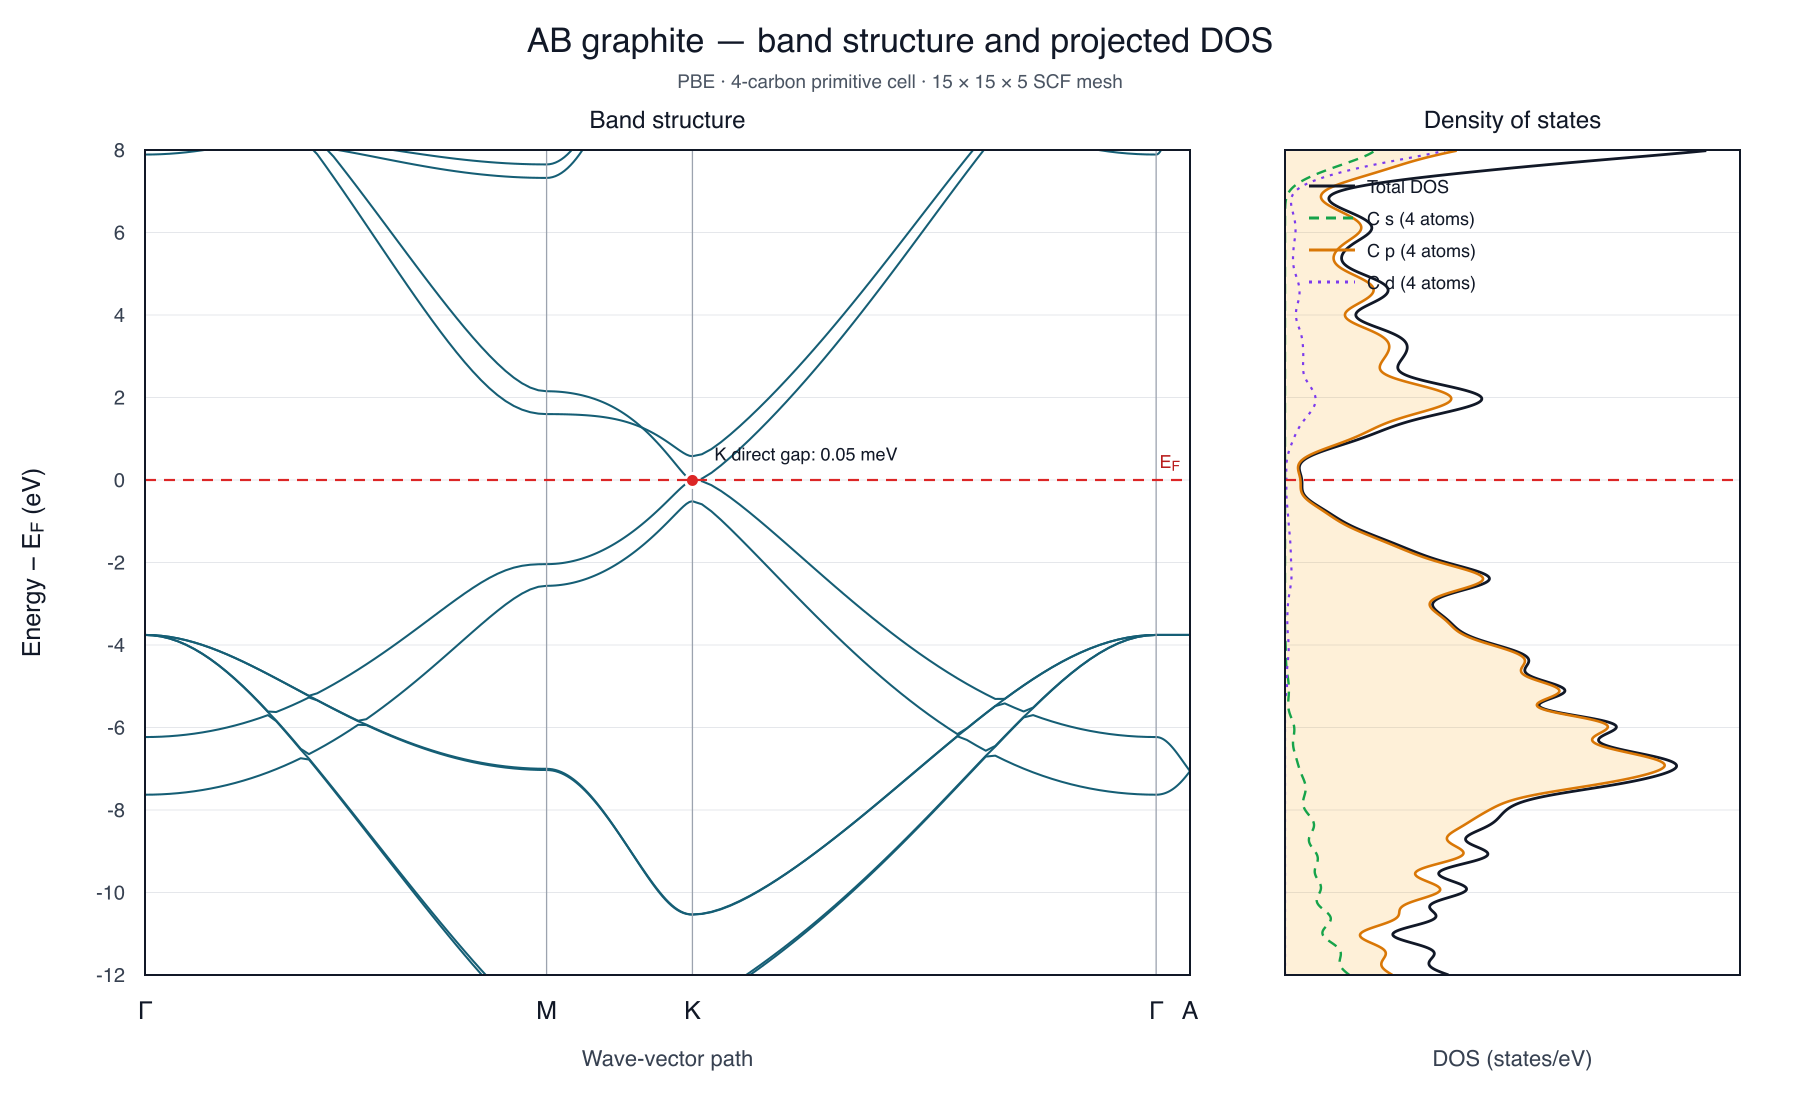
\includegraphics[width=.49\textwidth]{figures/graphite_band_pdos.png}\hfill
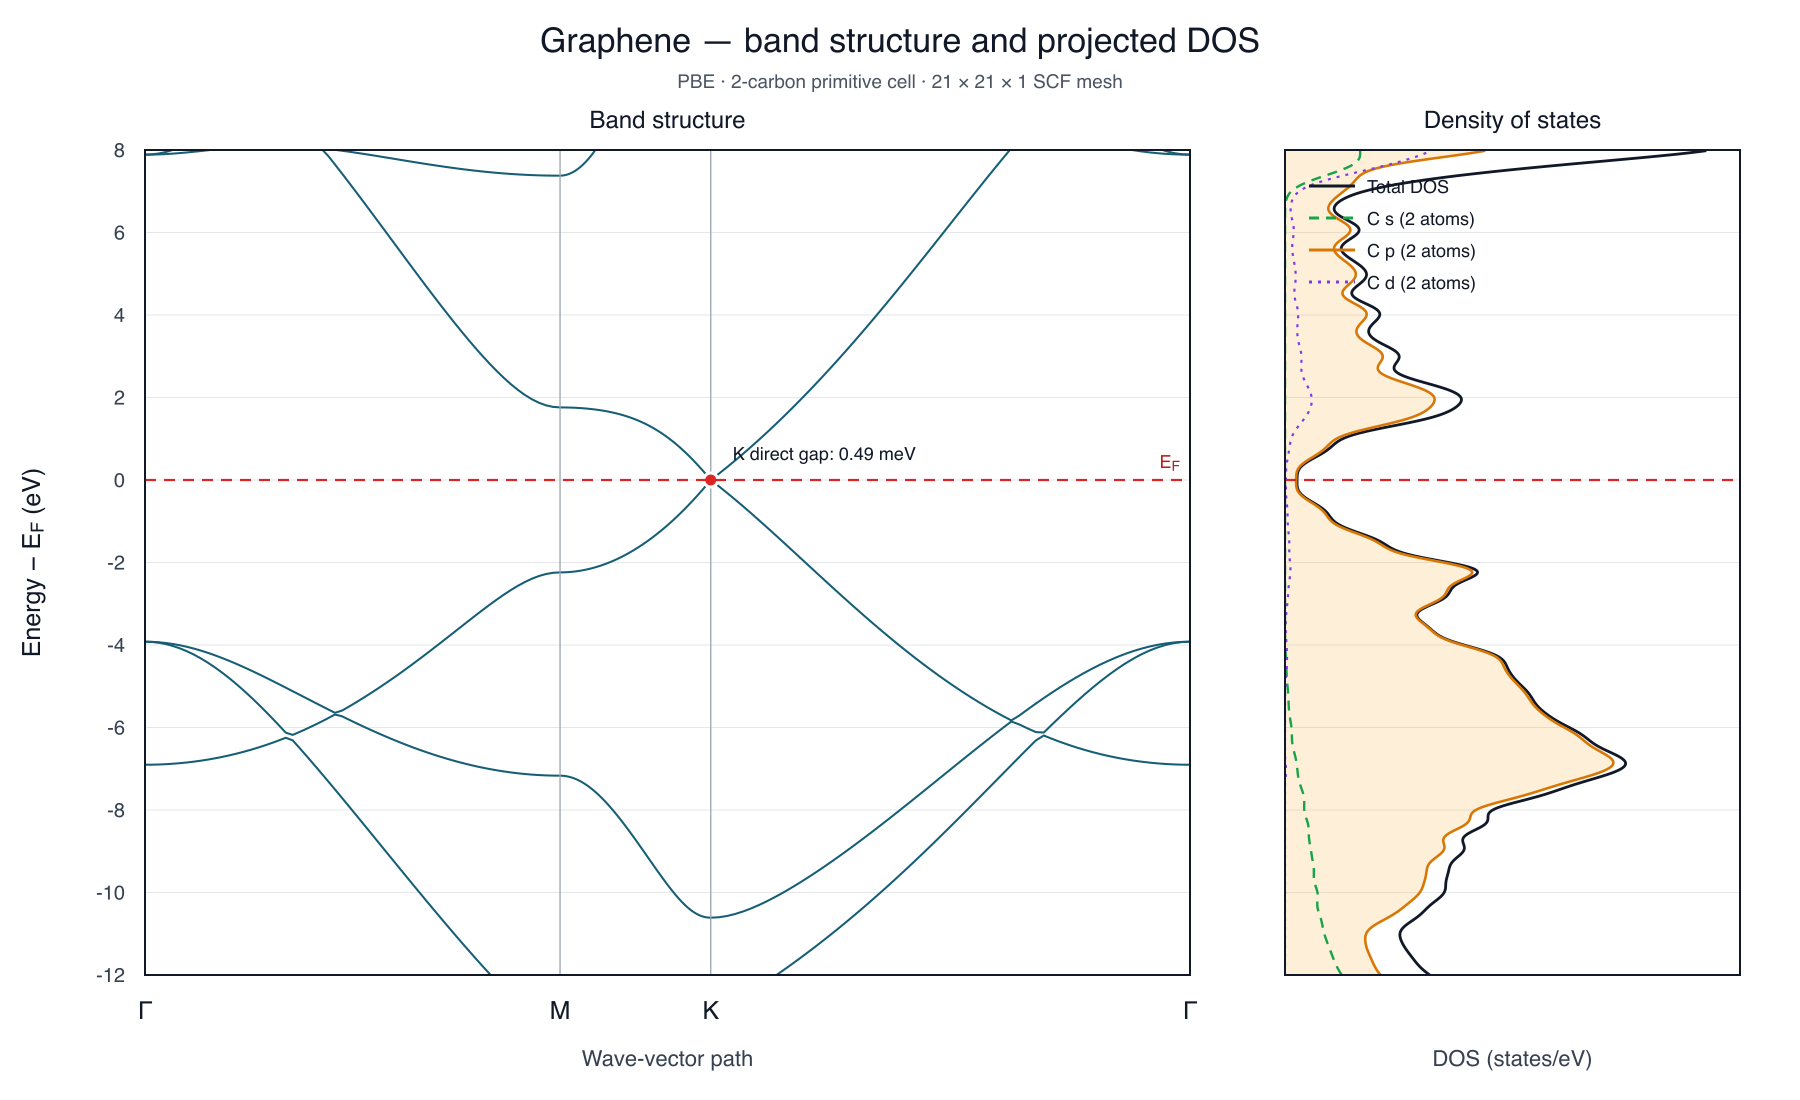
\includegraphics[width=.49\textwidth]{figures/graphene_band_pdos.png}
\caption{Test 010. AB graphite (left) and isolated graphene (right). The numerical K-point gaps are 0.052 and 0.493 meV; integrated valence counts are 16 and 8 electrons.}
\end{figure*}

\begin{figure*}[t]
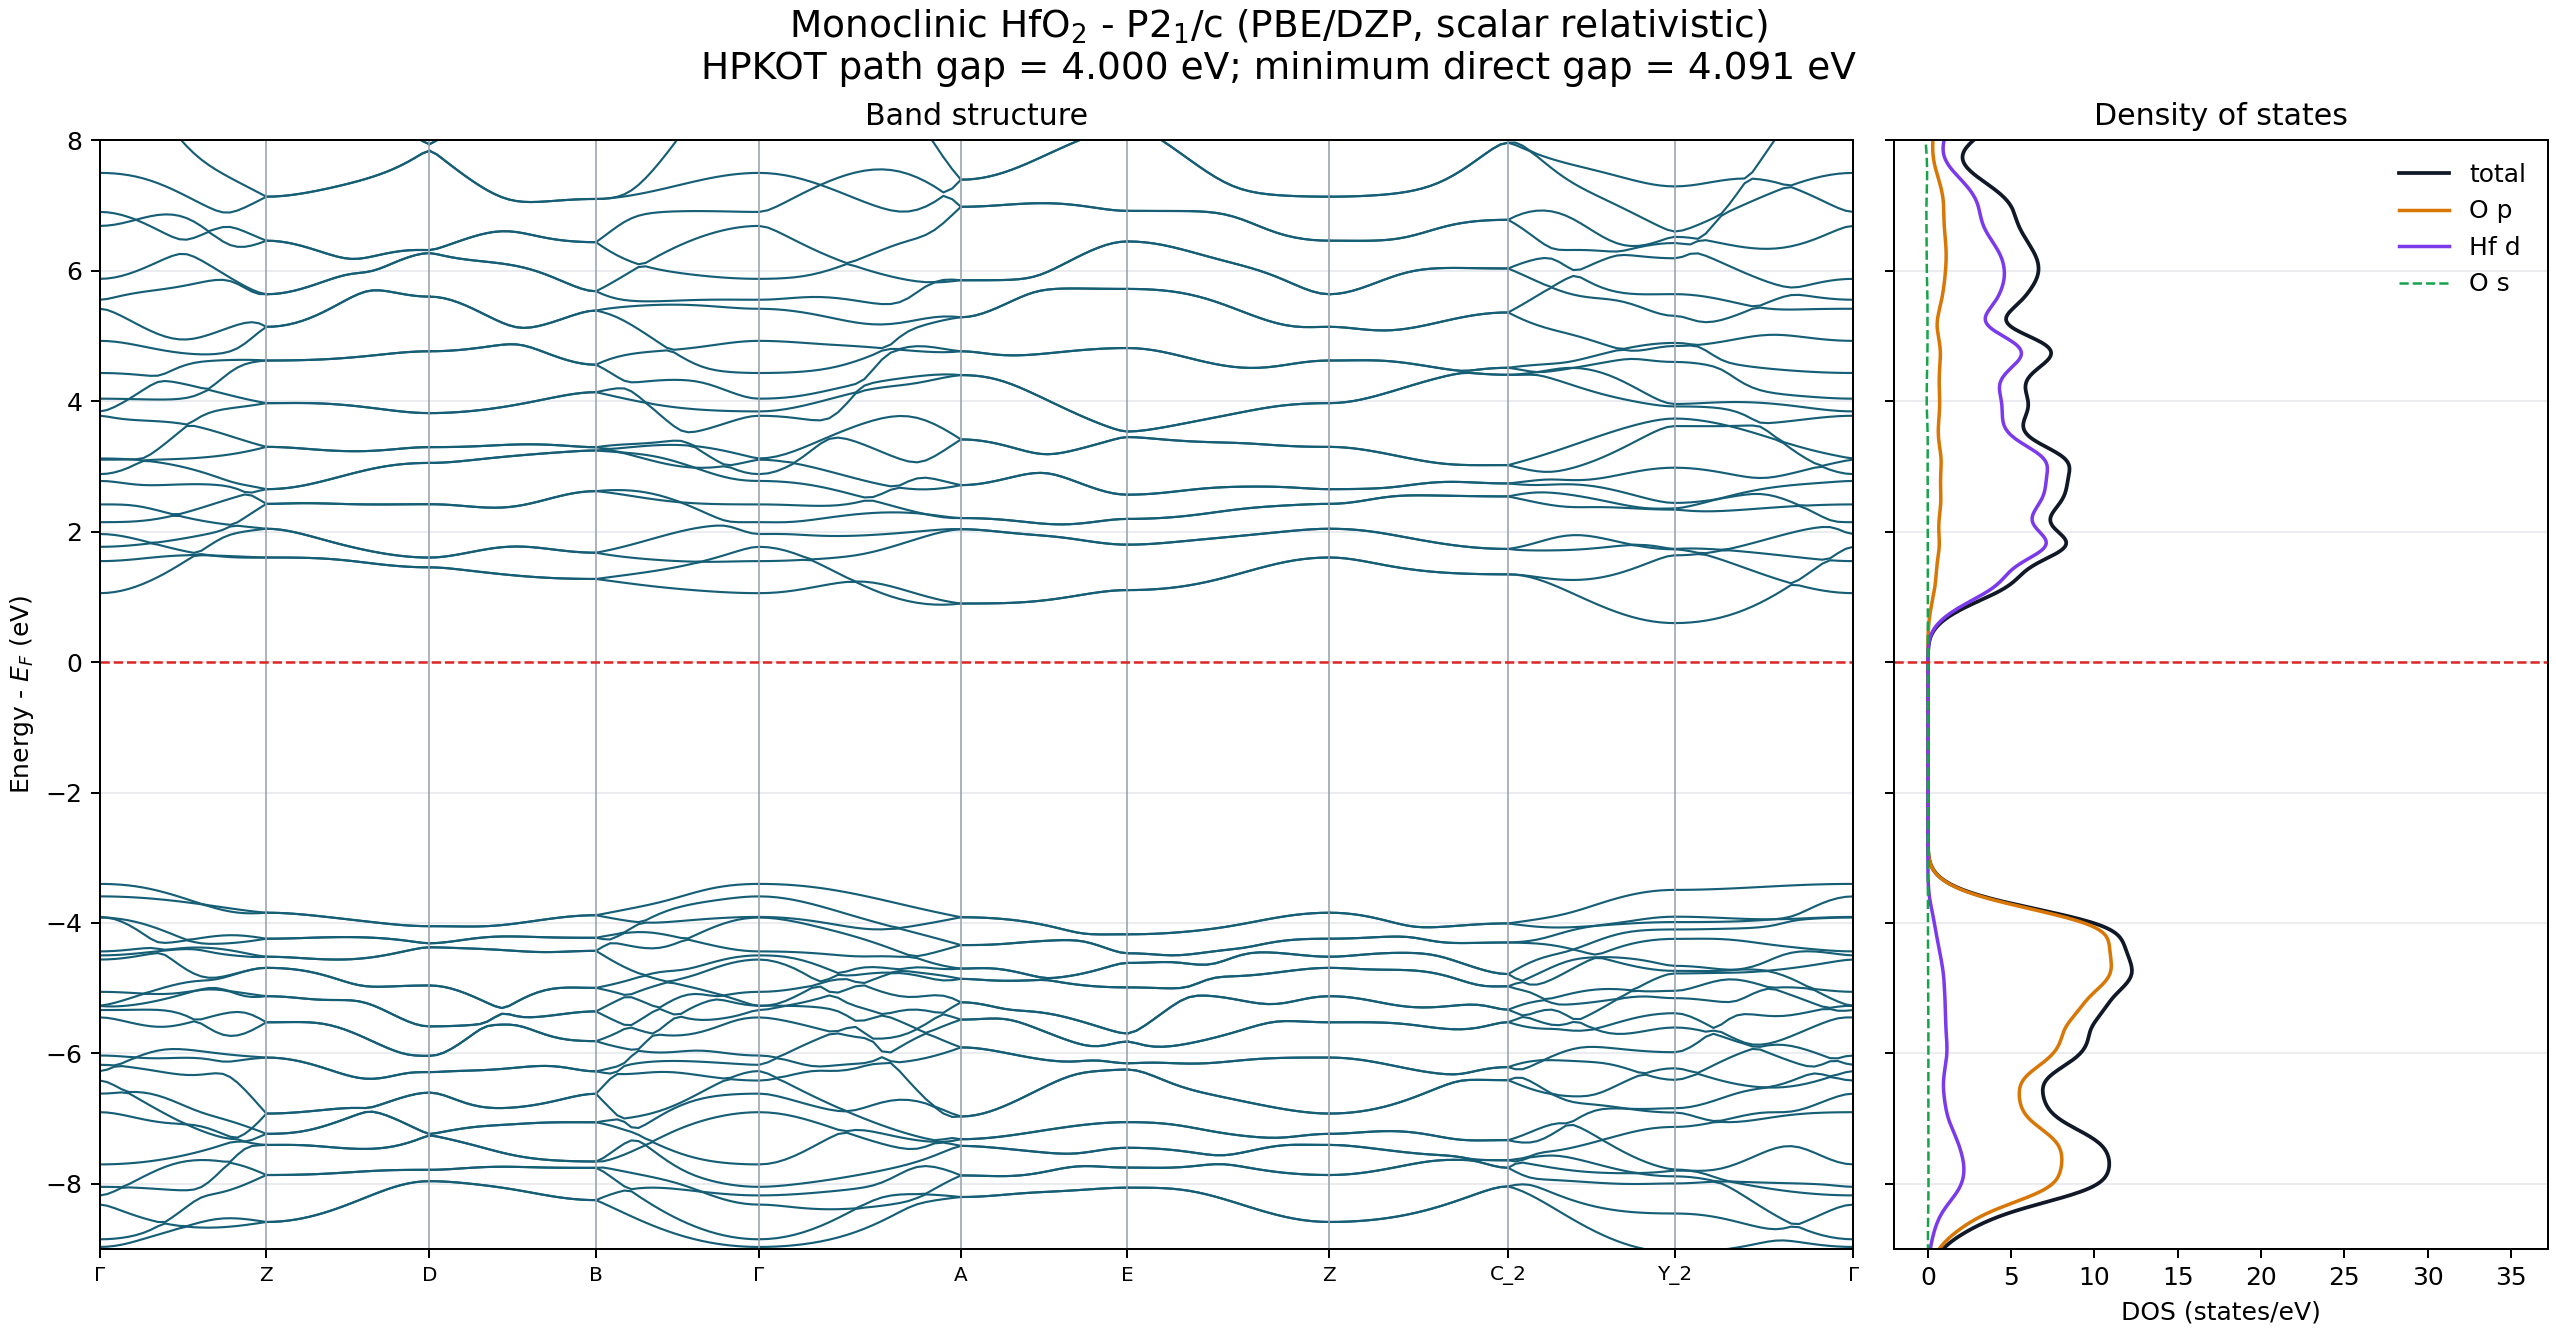
\includegraphics[width=.49\textwidth]{figures/hfo2_band_pdos.png}\hfill
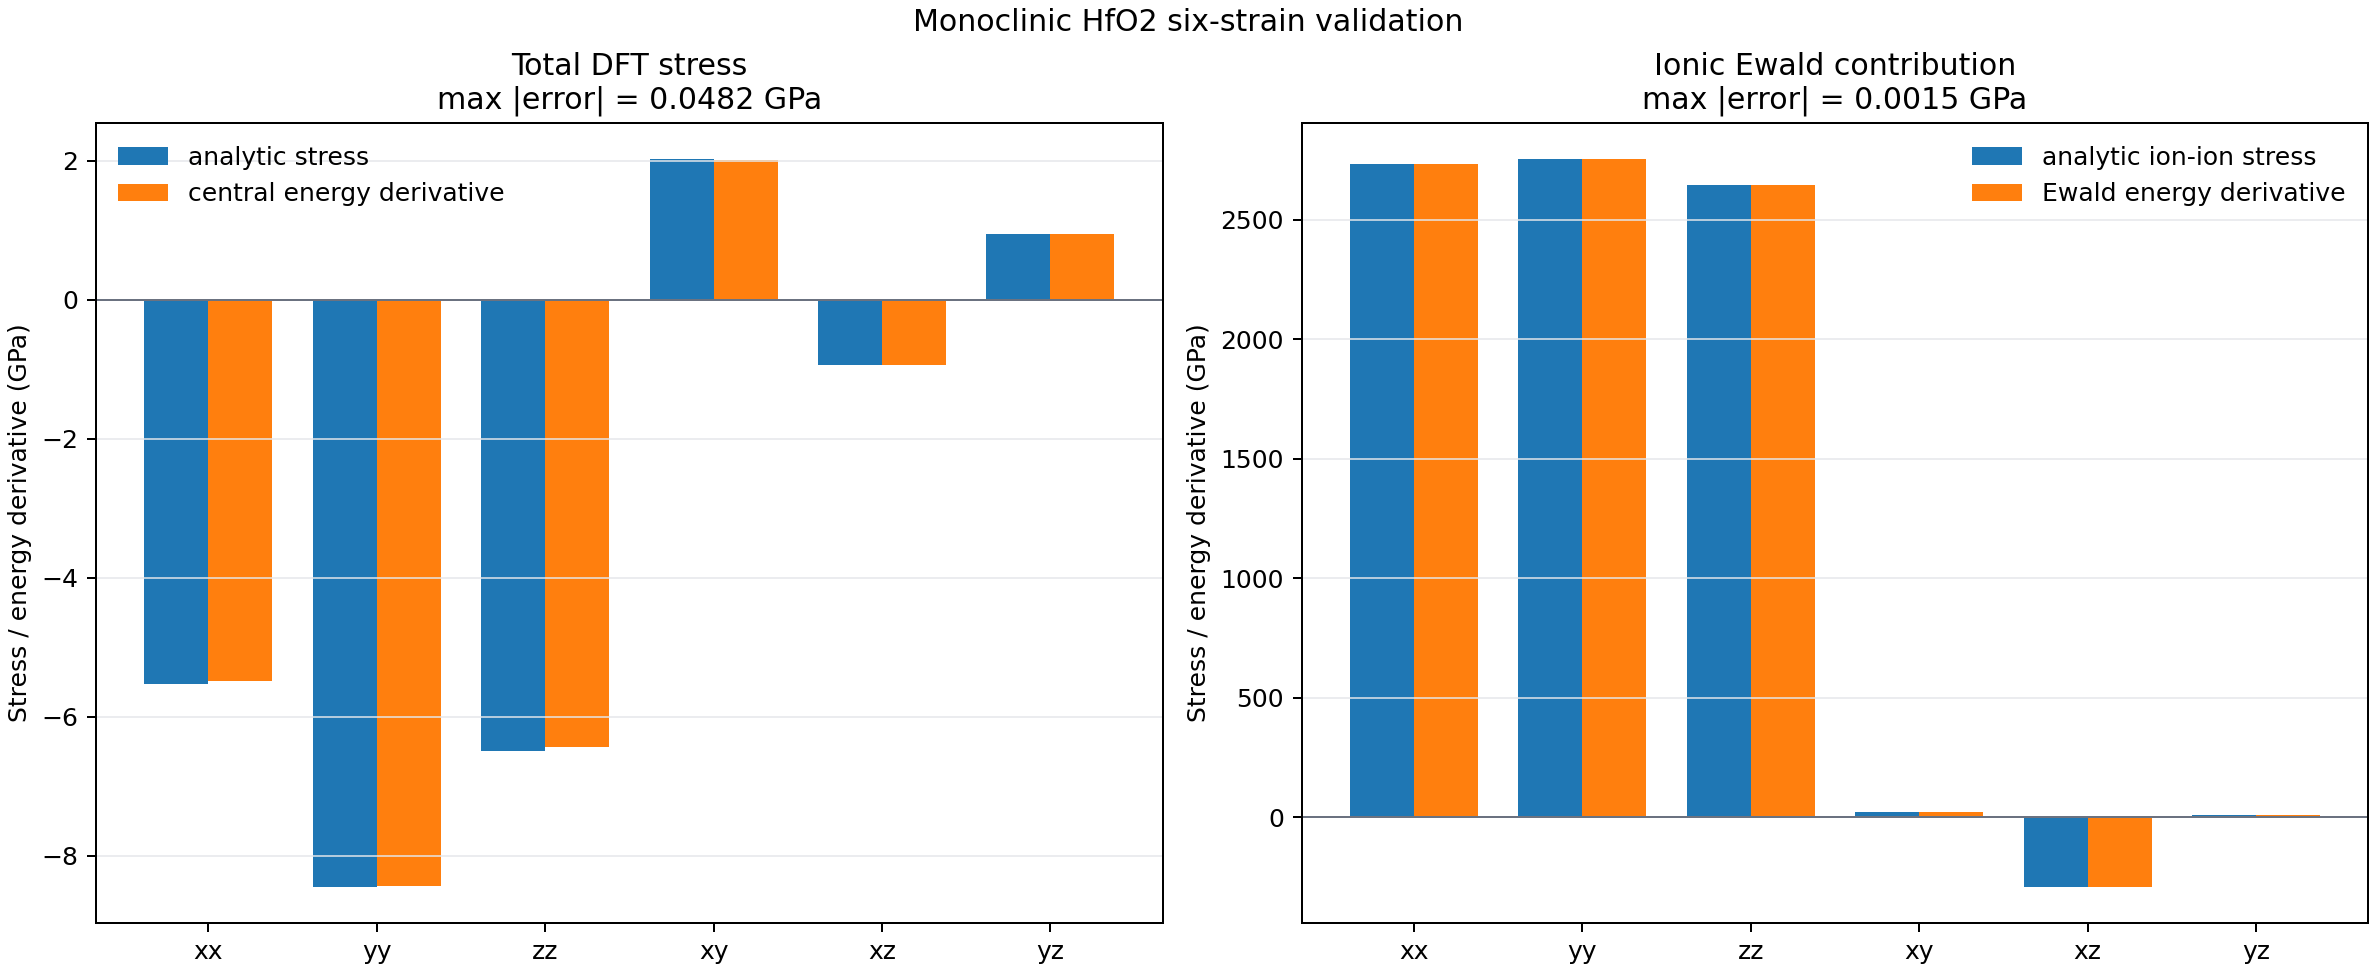
\includegraphics[width=.49\textwidth]{figures/hfo2_stress_fd.png}
\caption{Test 011. Monoclinic HfO$_2$ bands/PDOS (left) and six-component Ewald stress finite differences (right). The latter directly probes the ionic general-cell derivative.}
\end{figure*}

\begin{figure*}[t]
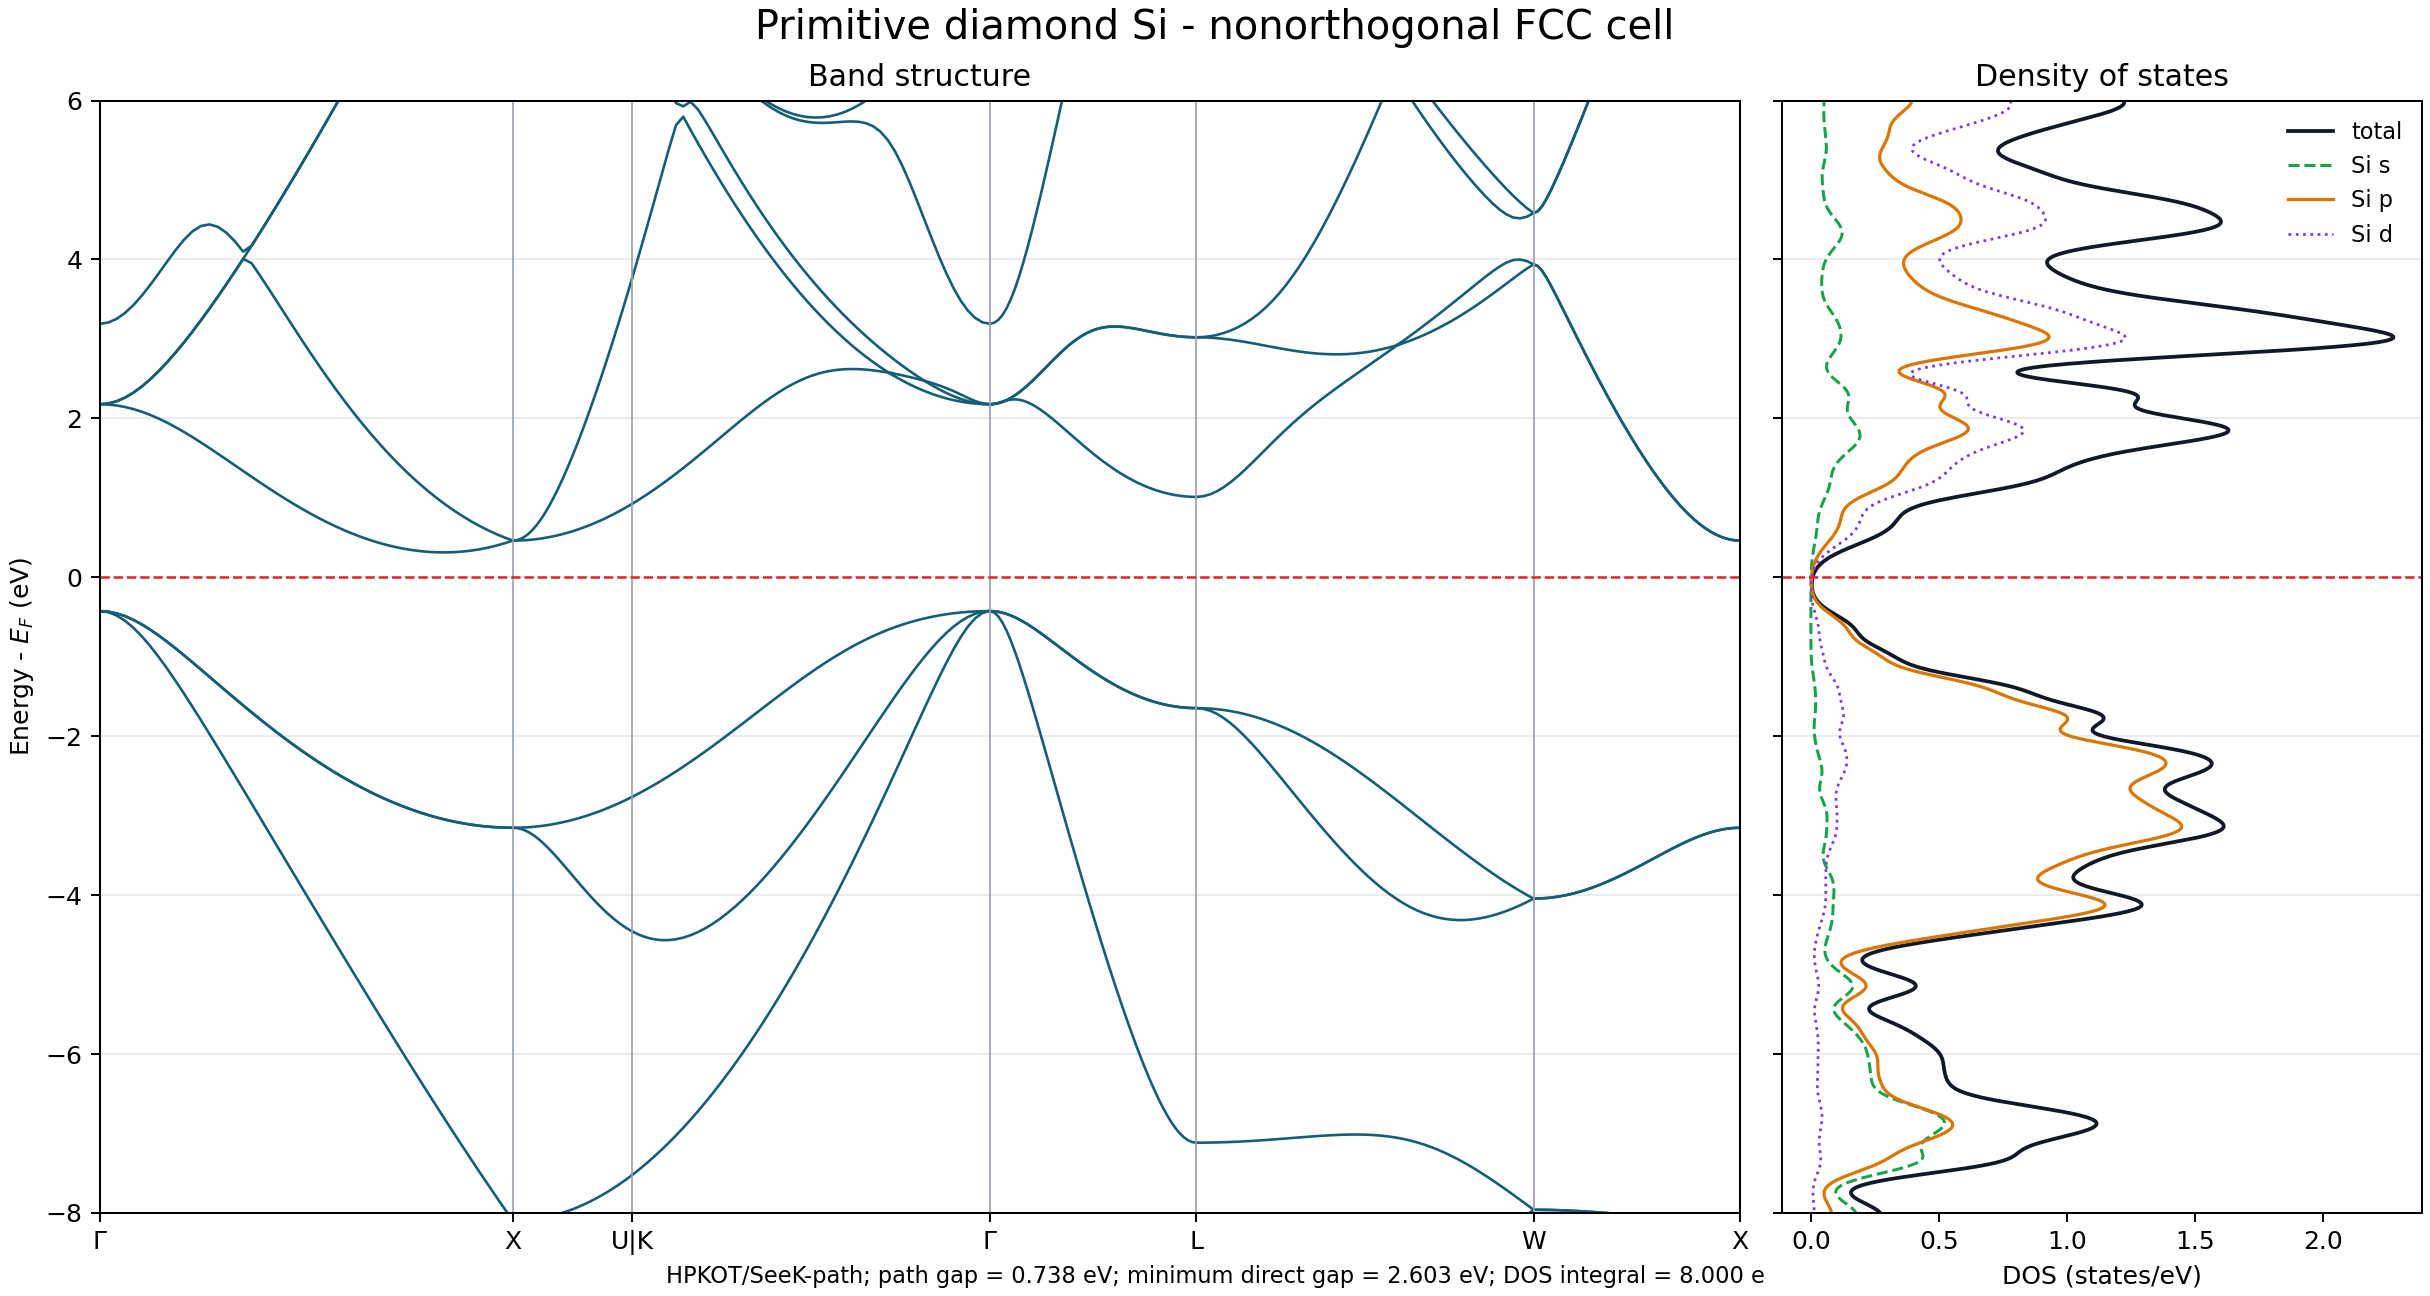
\includegraphics[width=.49\textwidth]{figures/si_band_pdos.png}\hfill
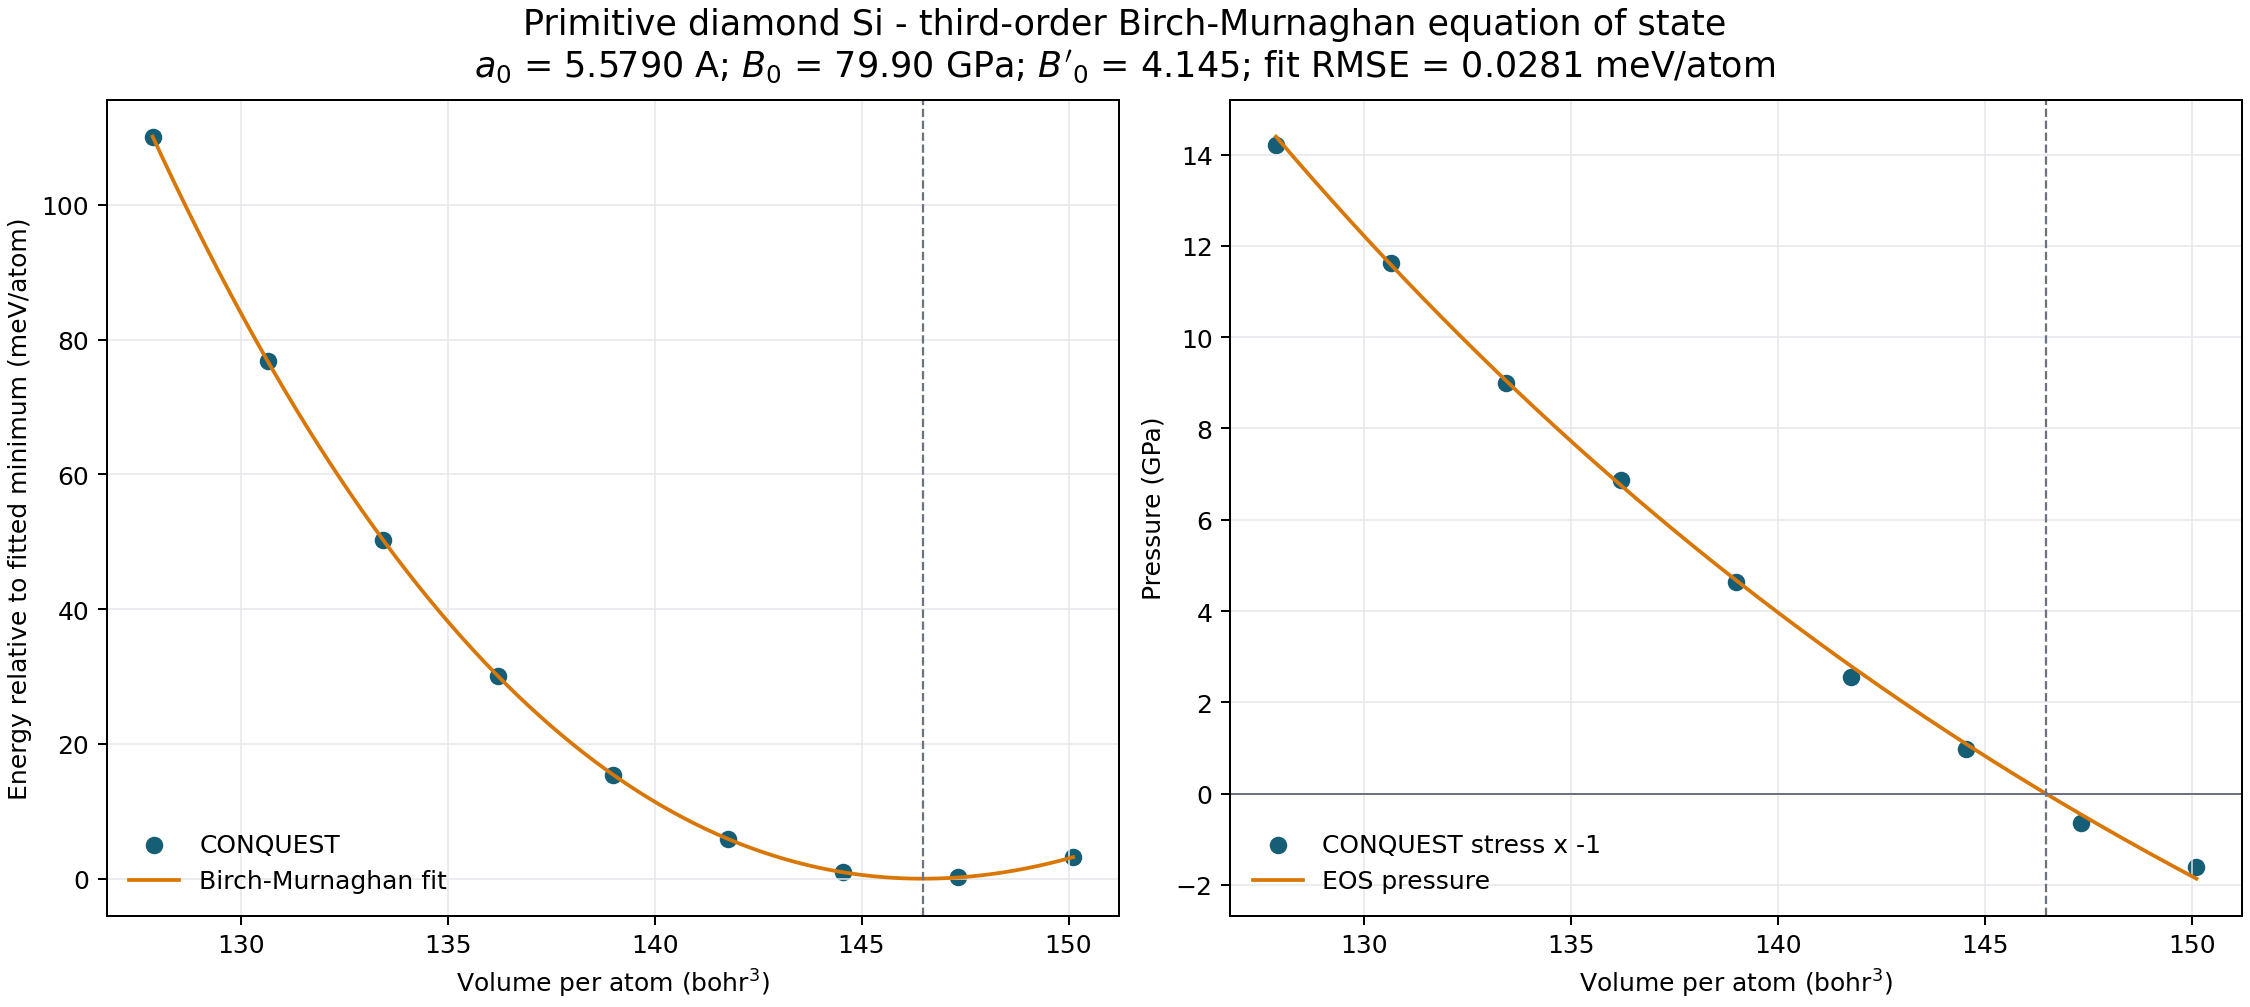
\includegraphics[width=.49\textwidth]{figures/si_eos.png}
\caption{Test 012. Primitive diamond-Si bands/PDOS (left; indirect path gap 0.7381 eV and 8.00046 integrated electrons) and nine-point Birch--Murnaghan EOS (right).}
\end{figure*}

\begin{figure*}[t]
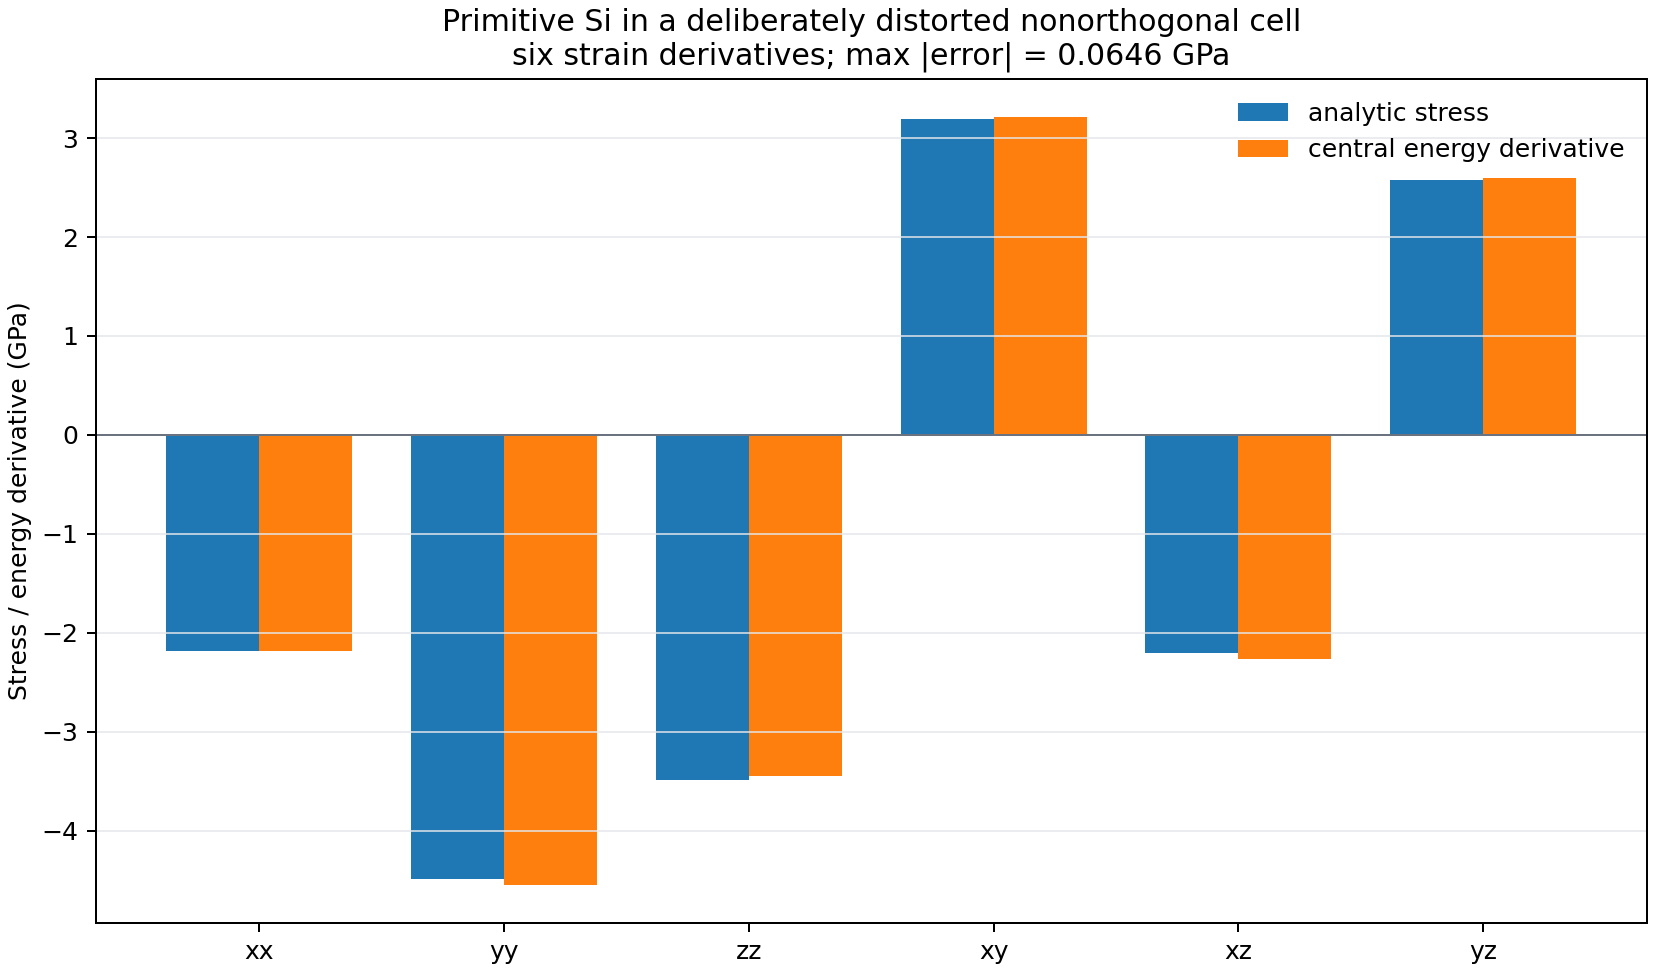
\includegraphics[width=.49\textwidth]{figures/si_stress_fd.png}\hfill
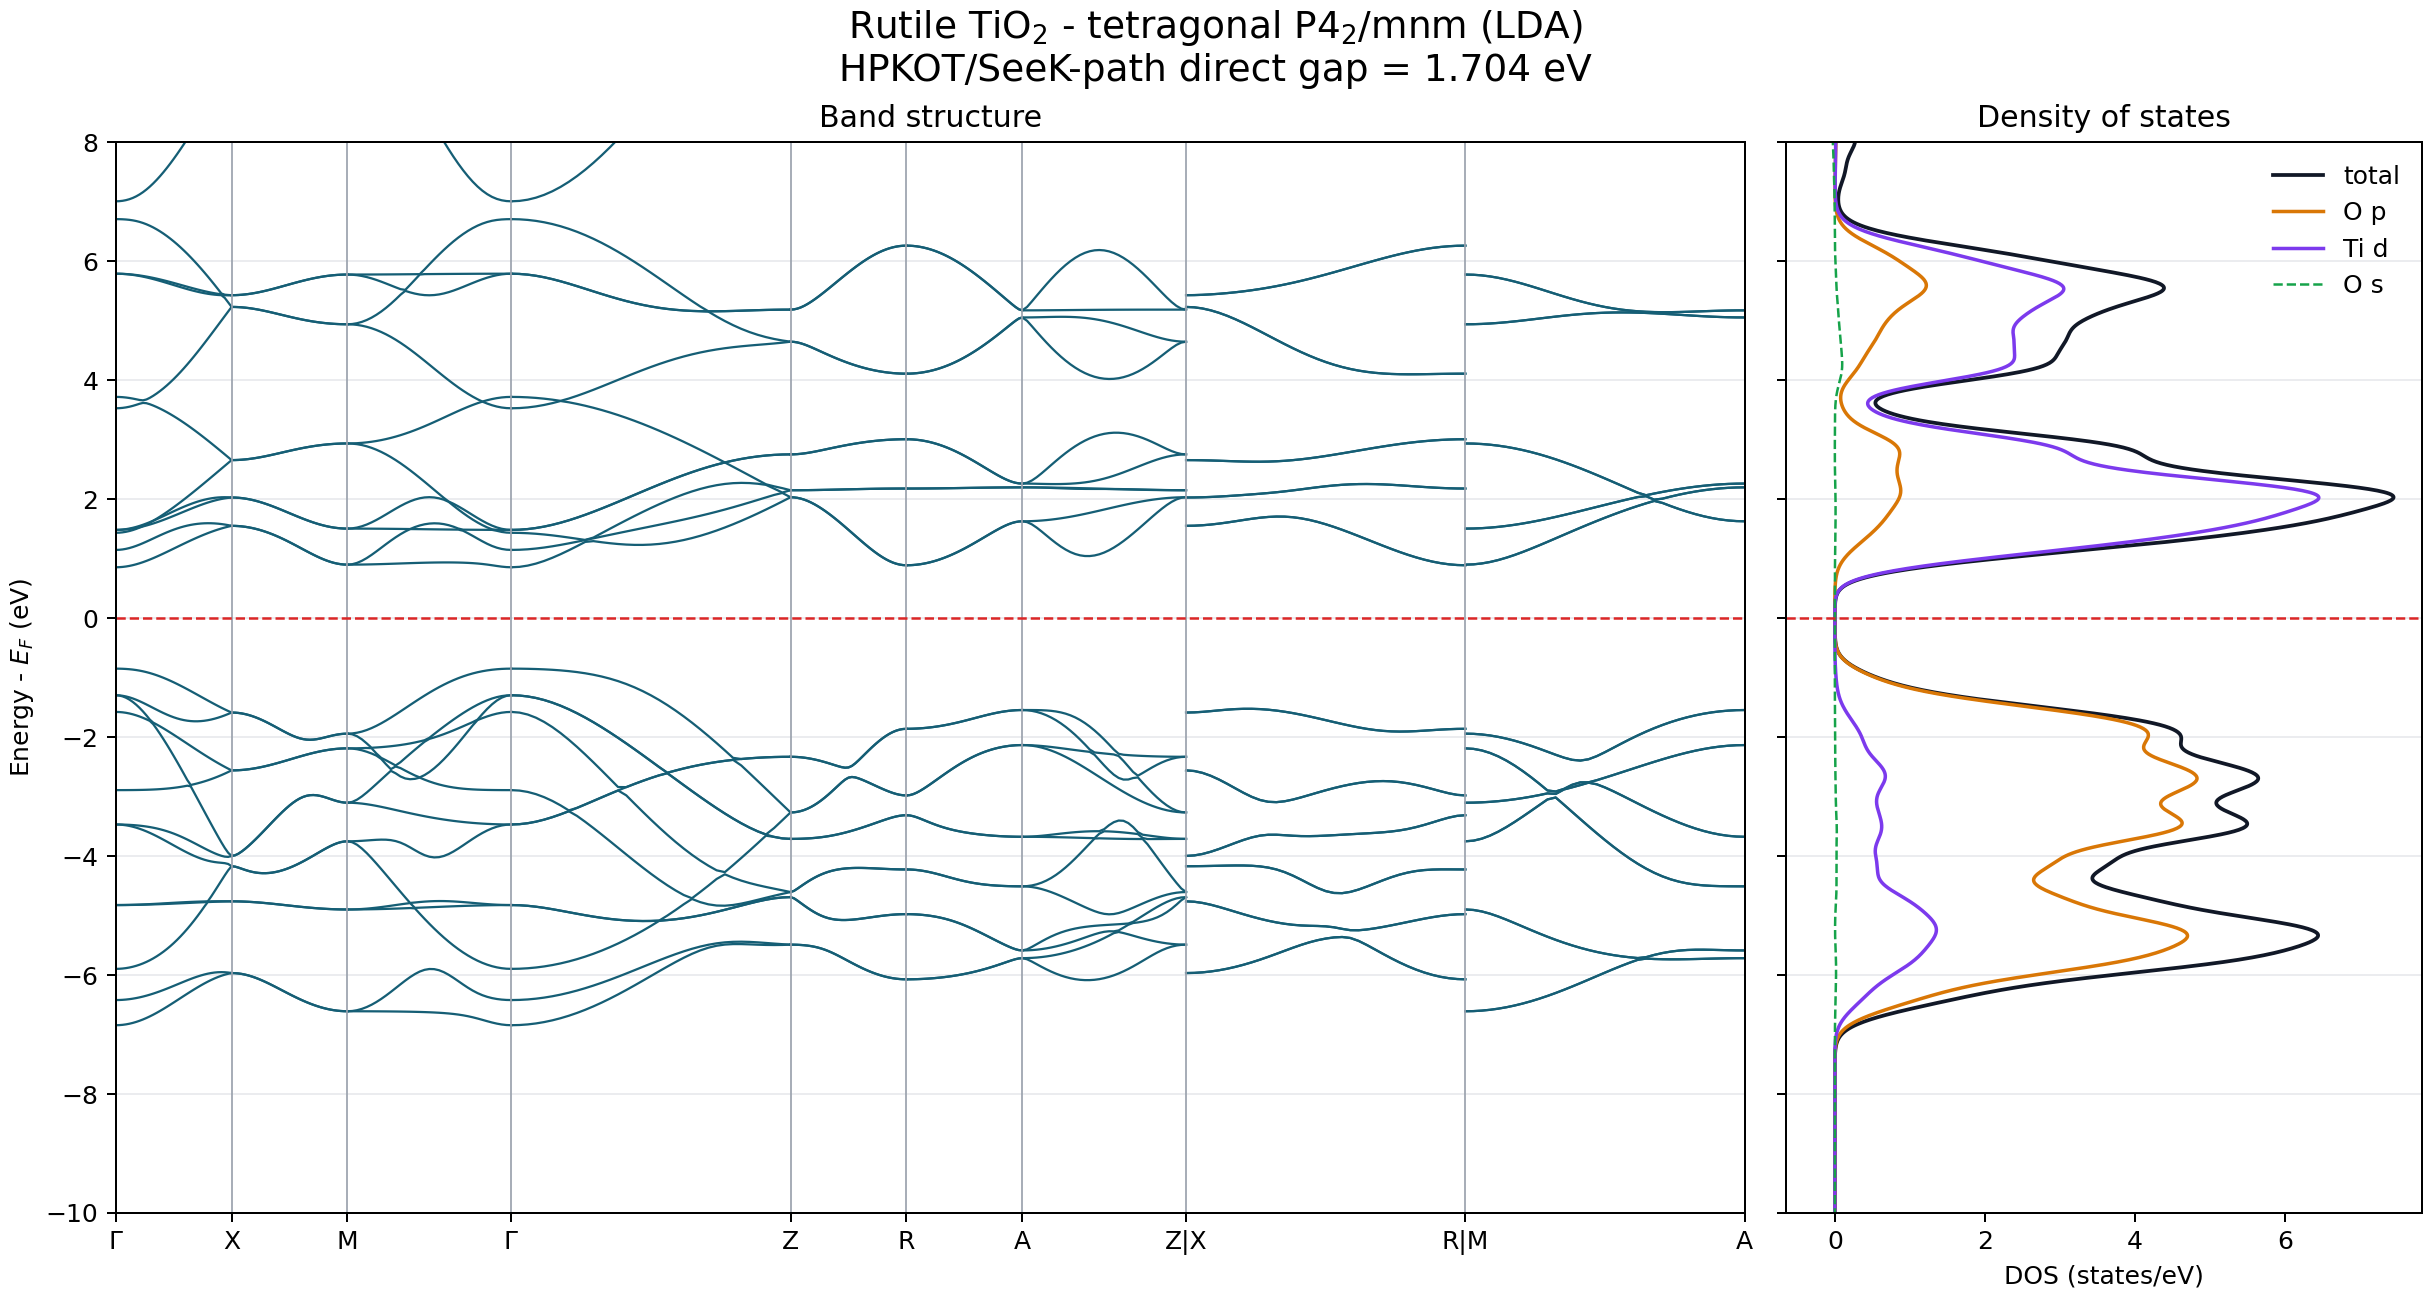
\includegraphics[width=.49\textwidth]{figures/rutile_band_pdos.png}
\caption{Six-strain primitive-Si stress validation (left) and Test-013 rutile TiO$_2$ bands/PDOS (right). Rutile provides an anisotropic right-angled control.}
\end{figure*}

\begin{figure*}[t]
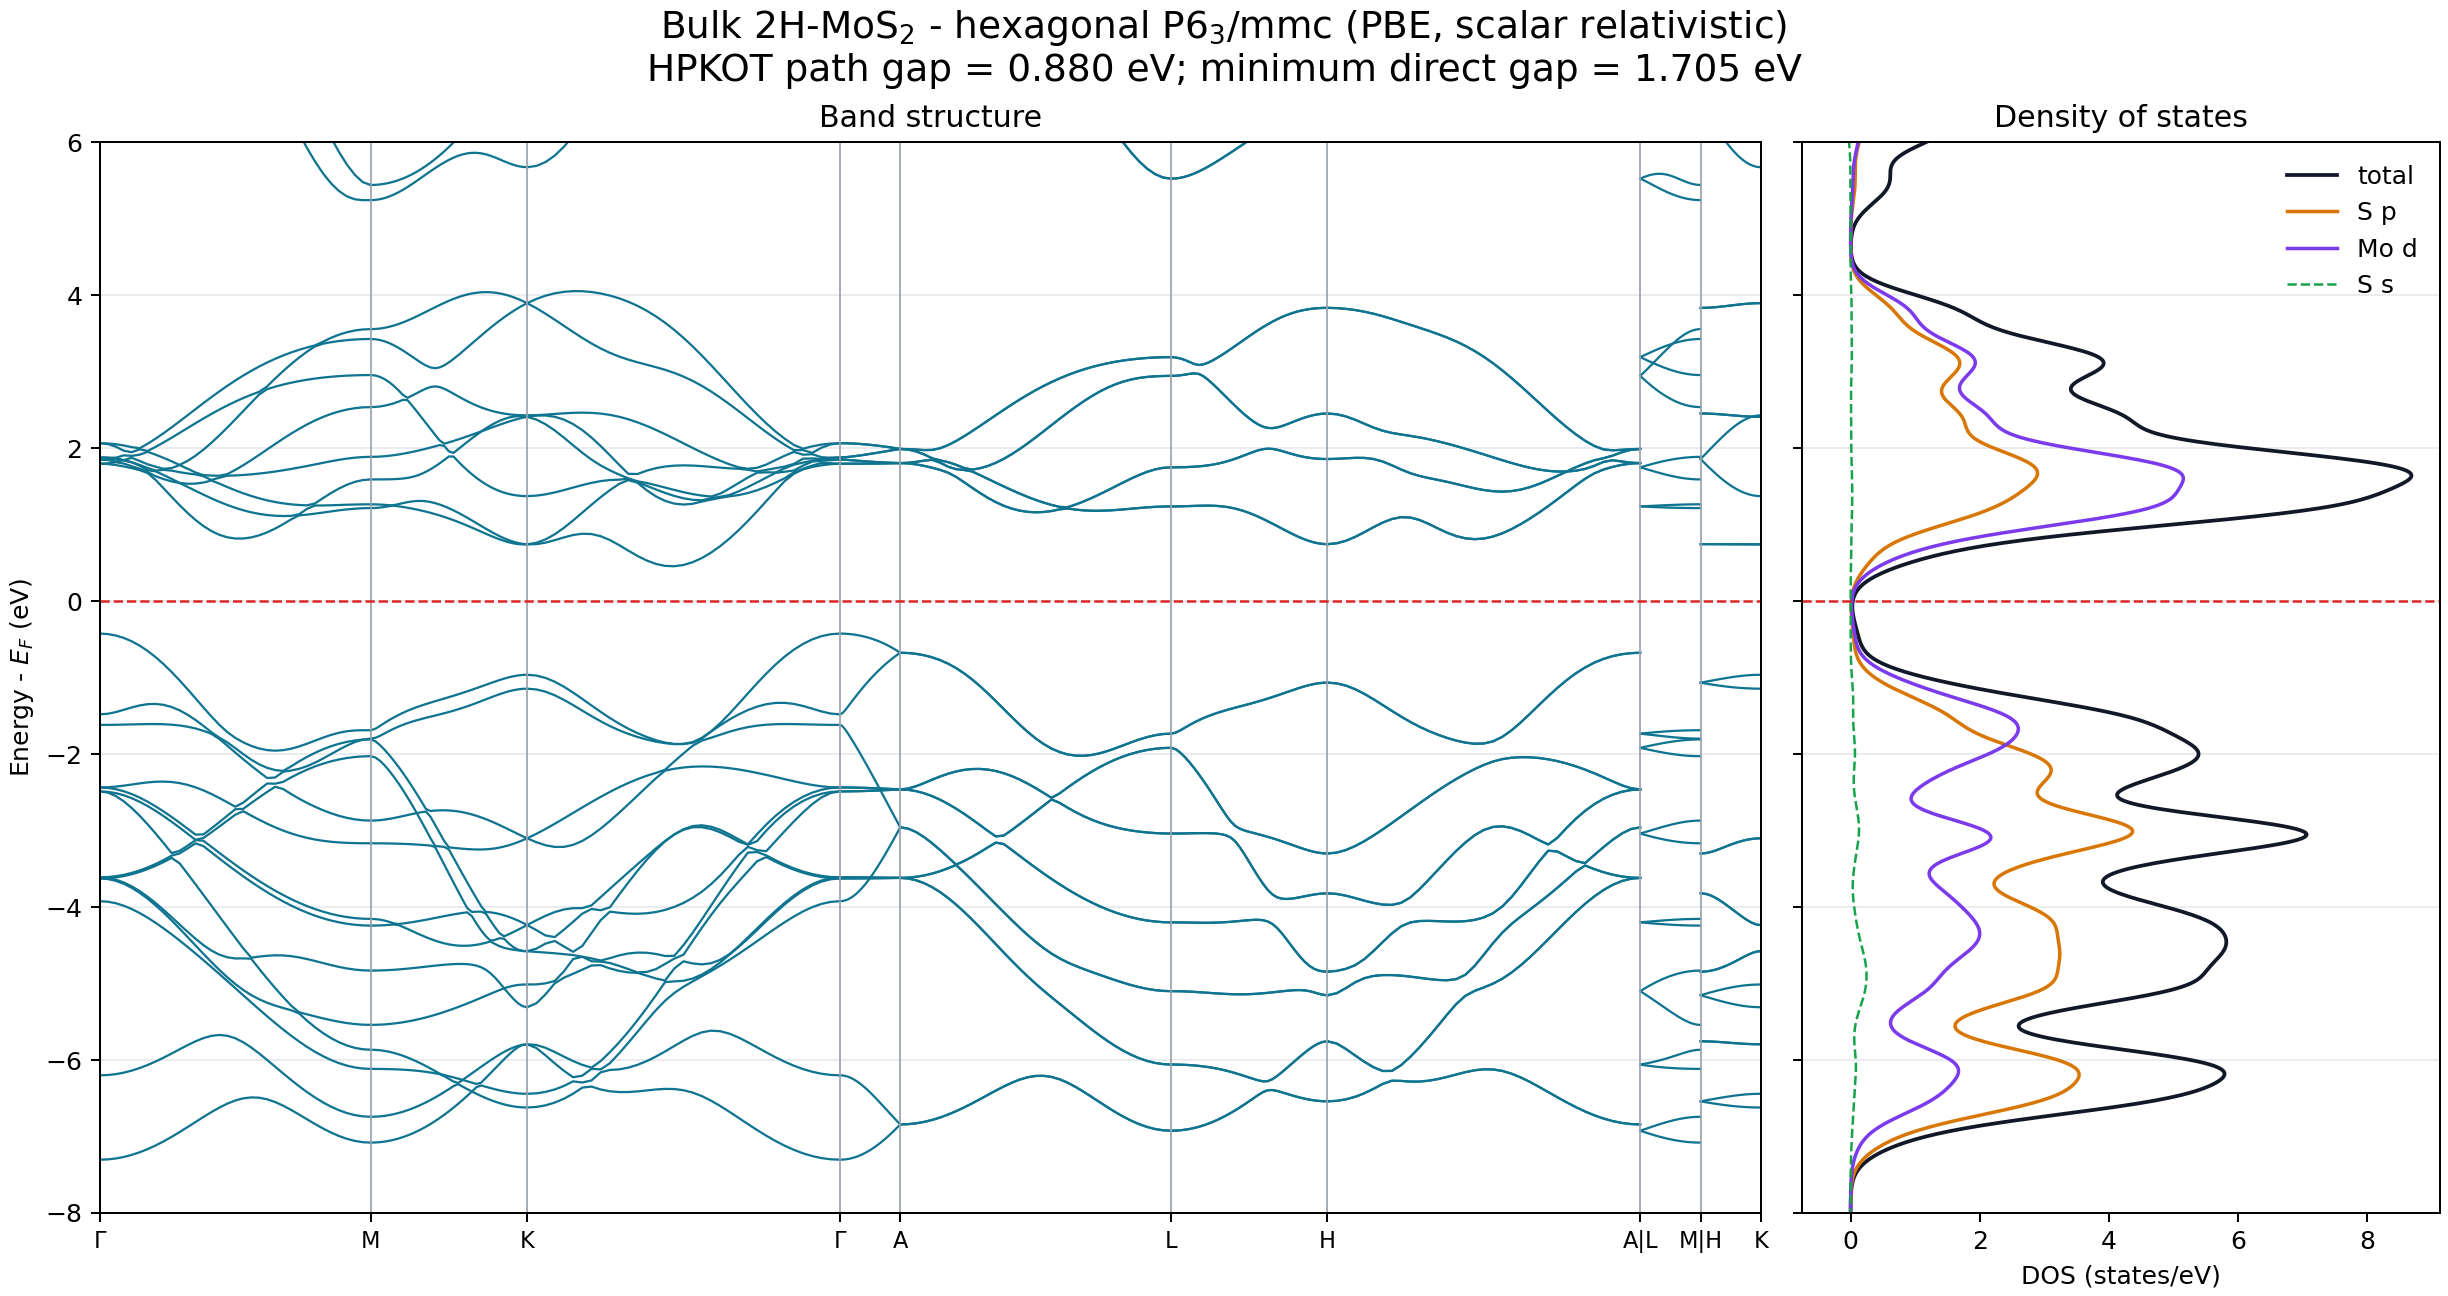
\includegraphics[width=.49\textwidth]{figures/mos2_band_pdos.png}\hfill
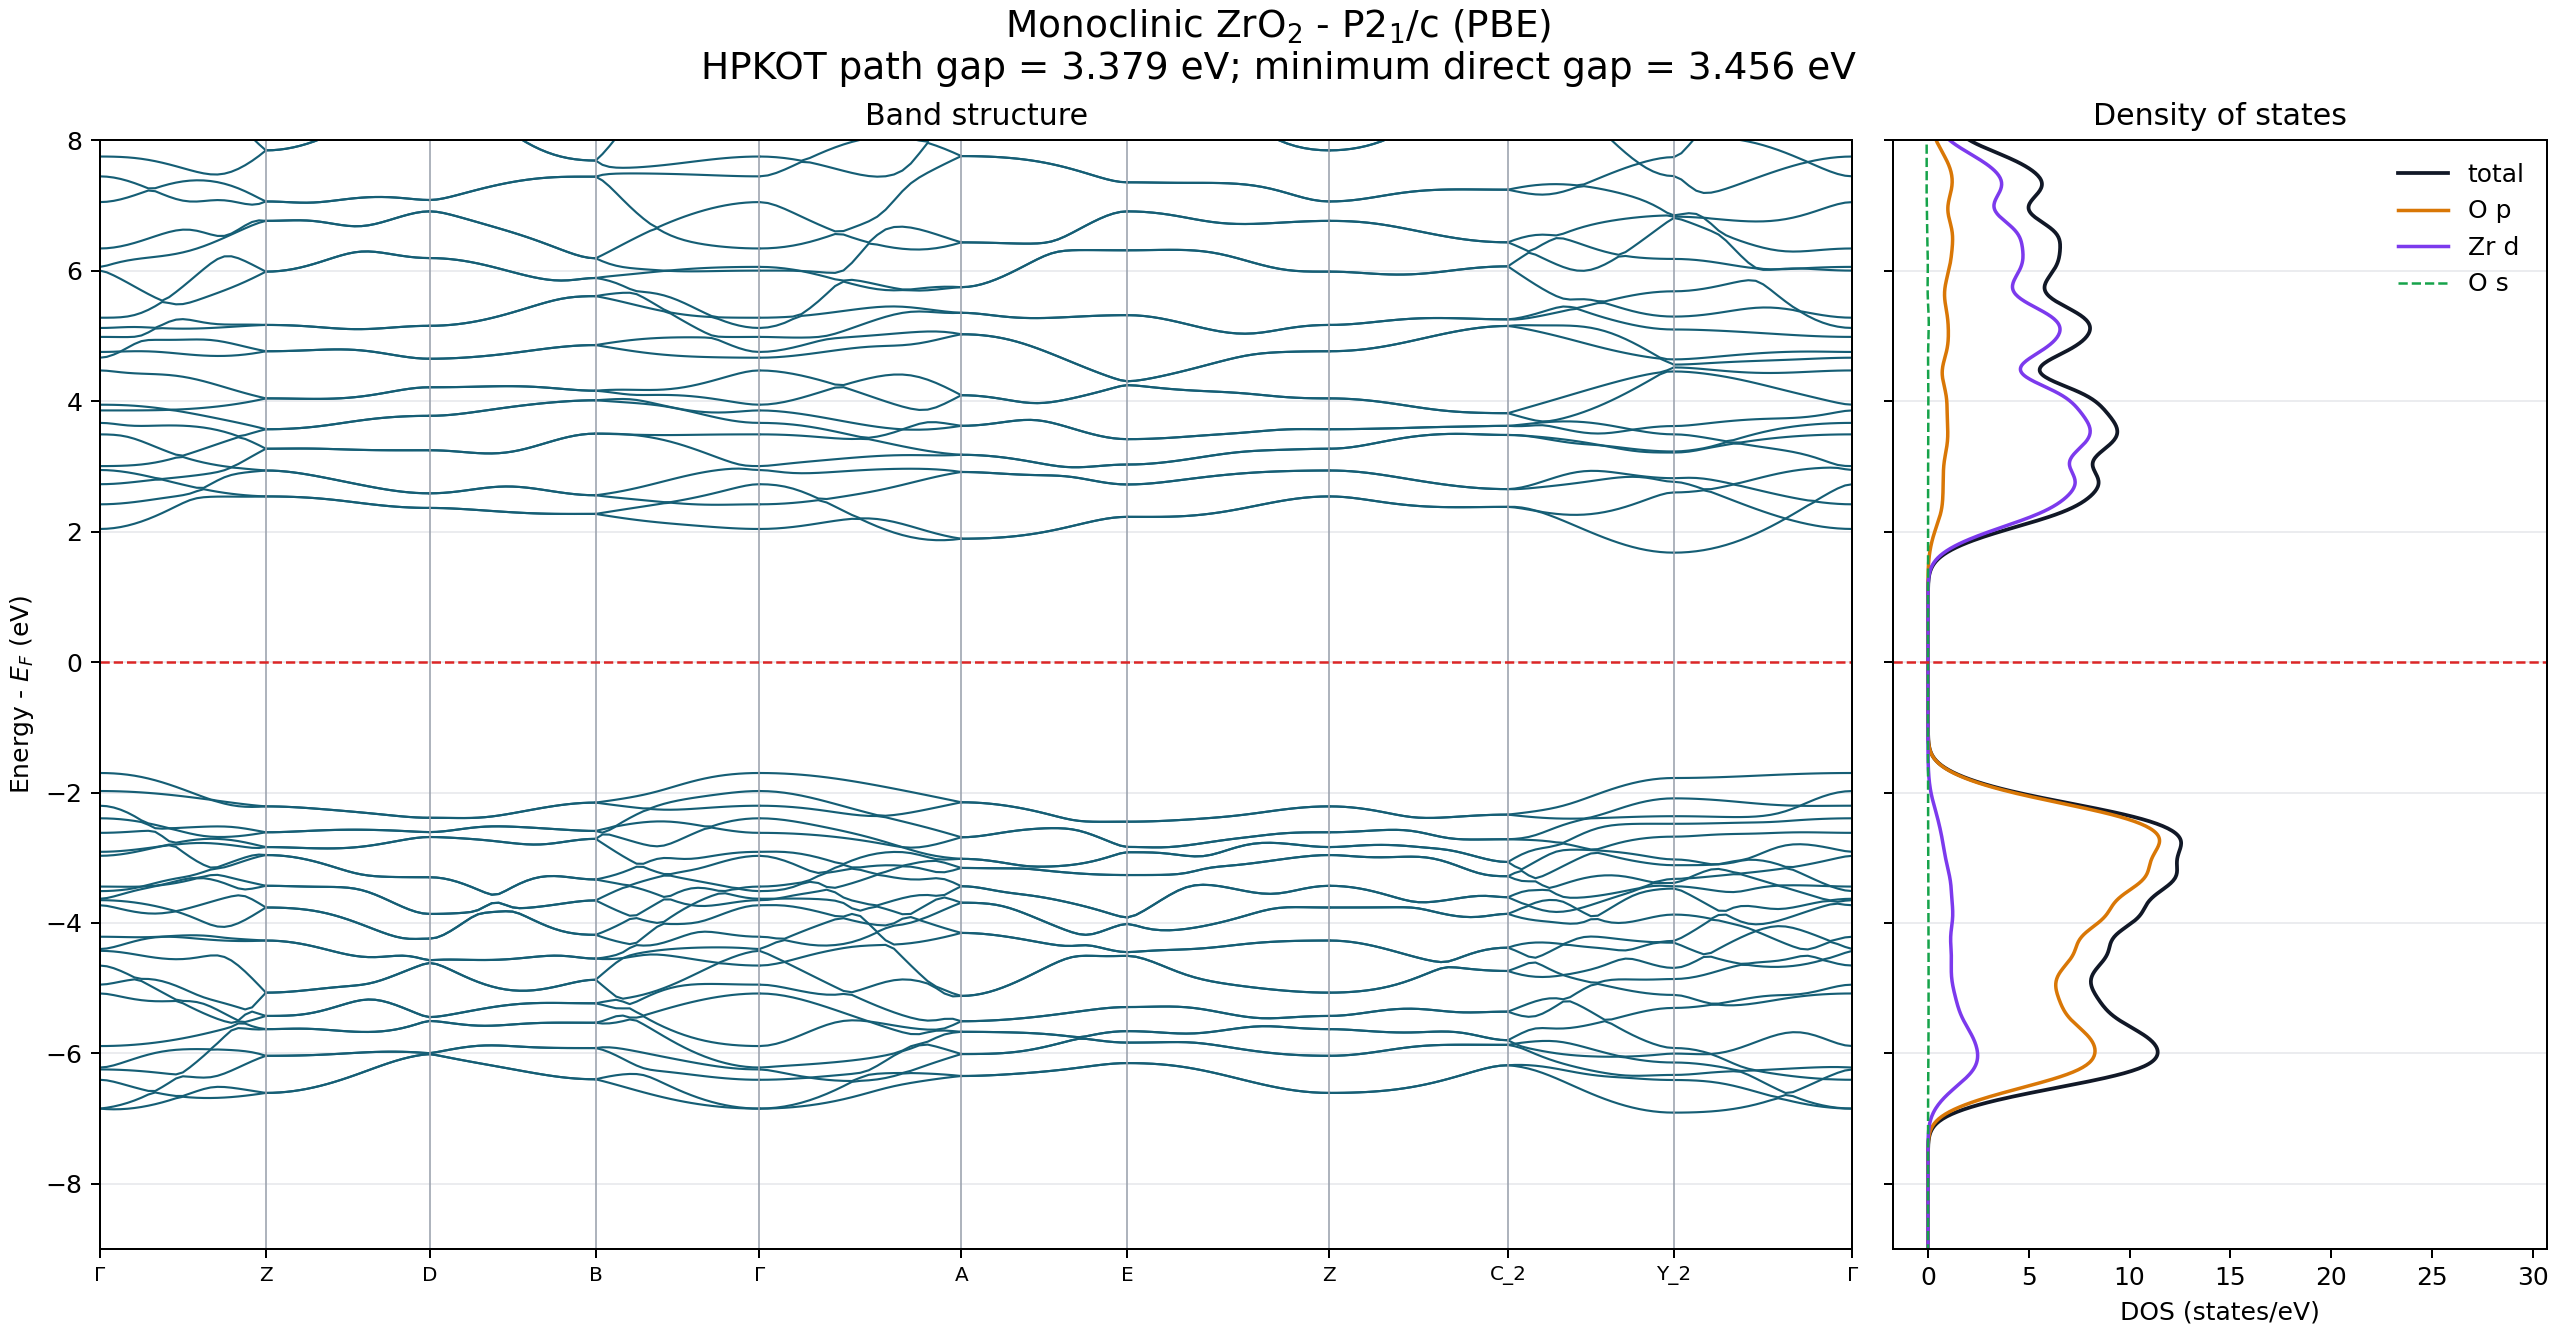
\includegraphics[width=.49\textwidth]{figures/zro2_band_pdos.png}
\caption{Tests 014 and 015. Bulk 2H-MoS$_2$ (left; indirect path gap 0.8804 eV) and monoclinic ZrO$_2$ (right; indirect path gap 3.3789 eV), with orbital-resolved PDOS.}
\end{figure*}

\begin{figure*}[t]
\centering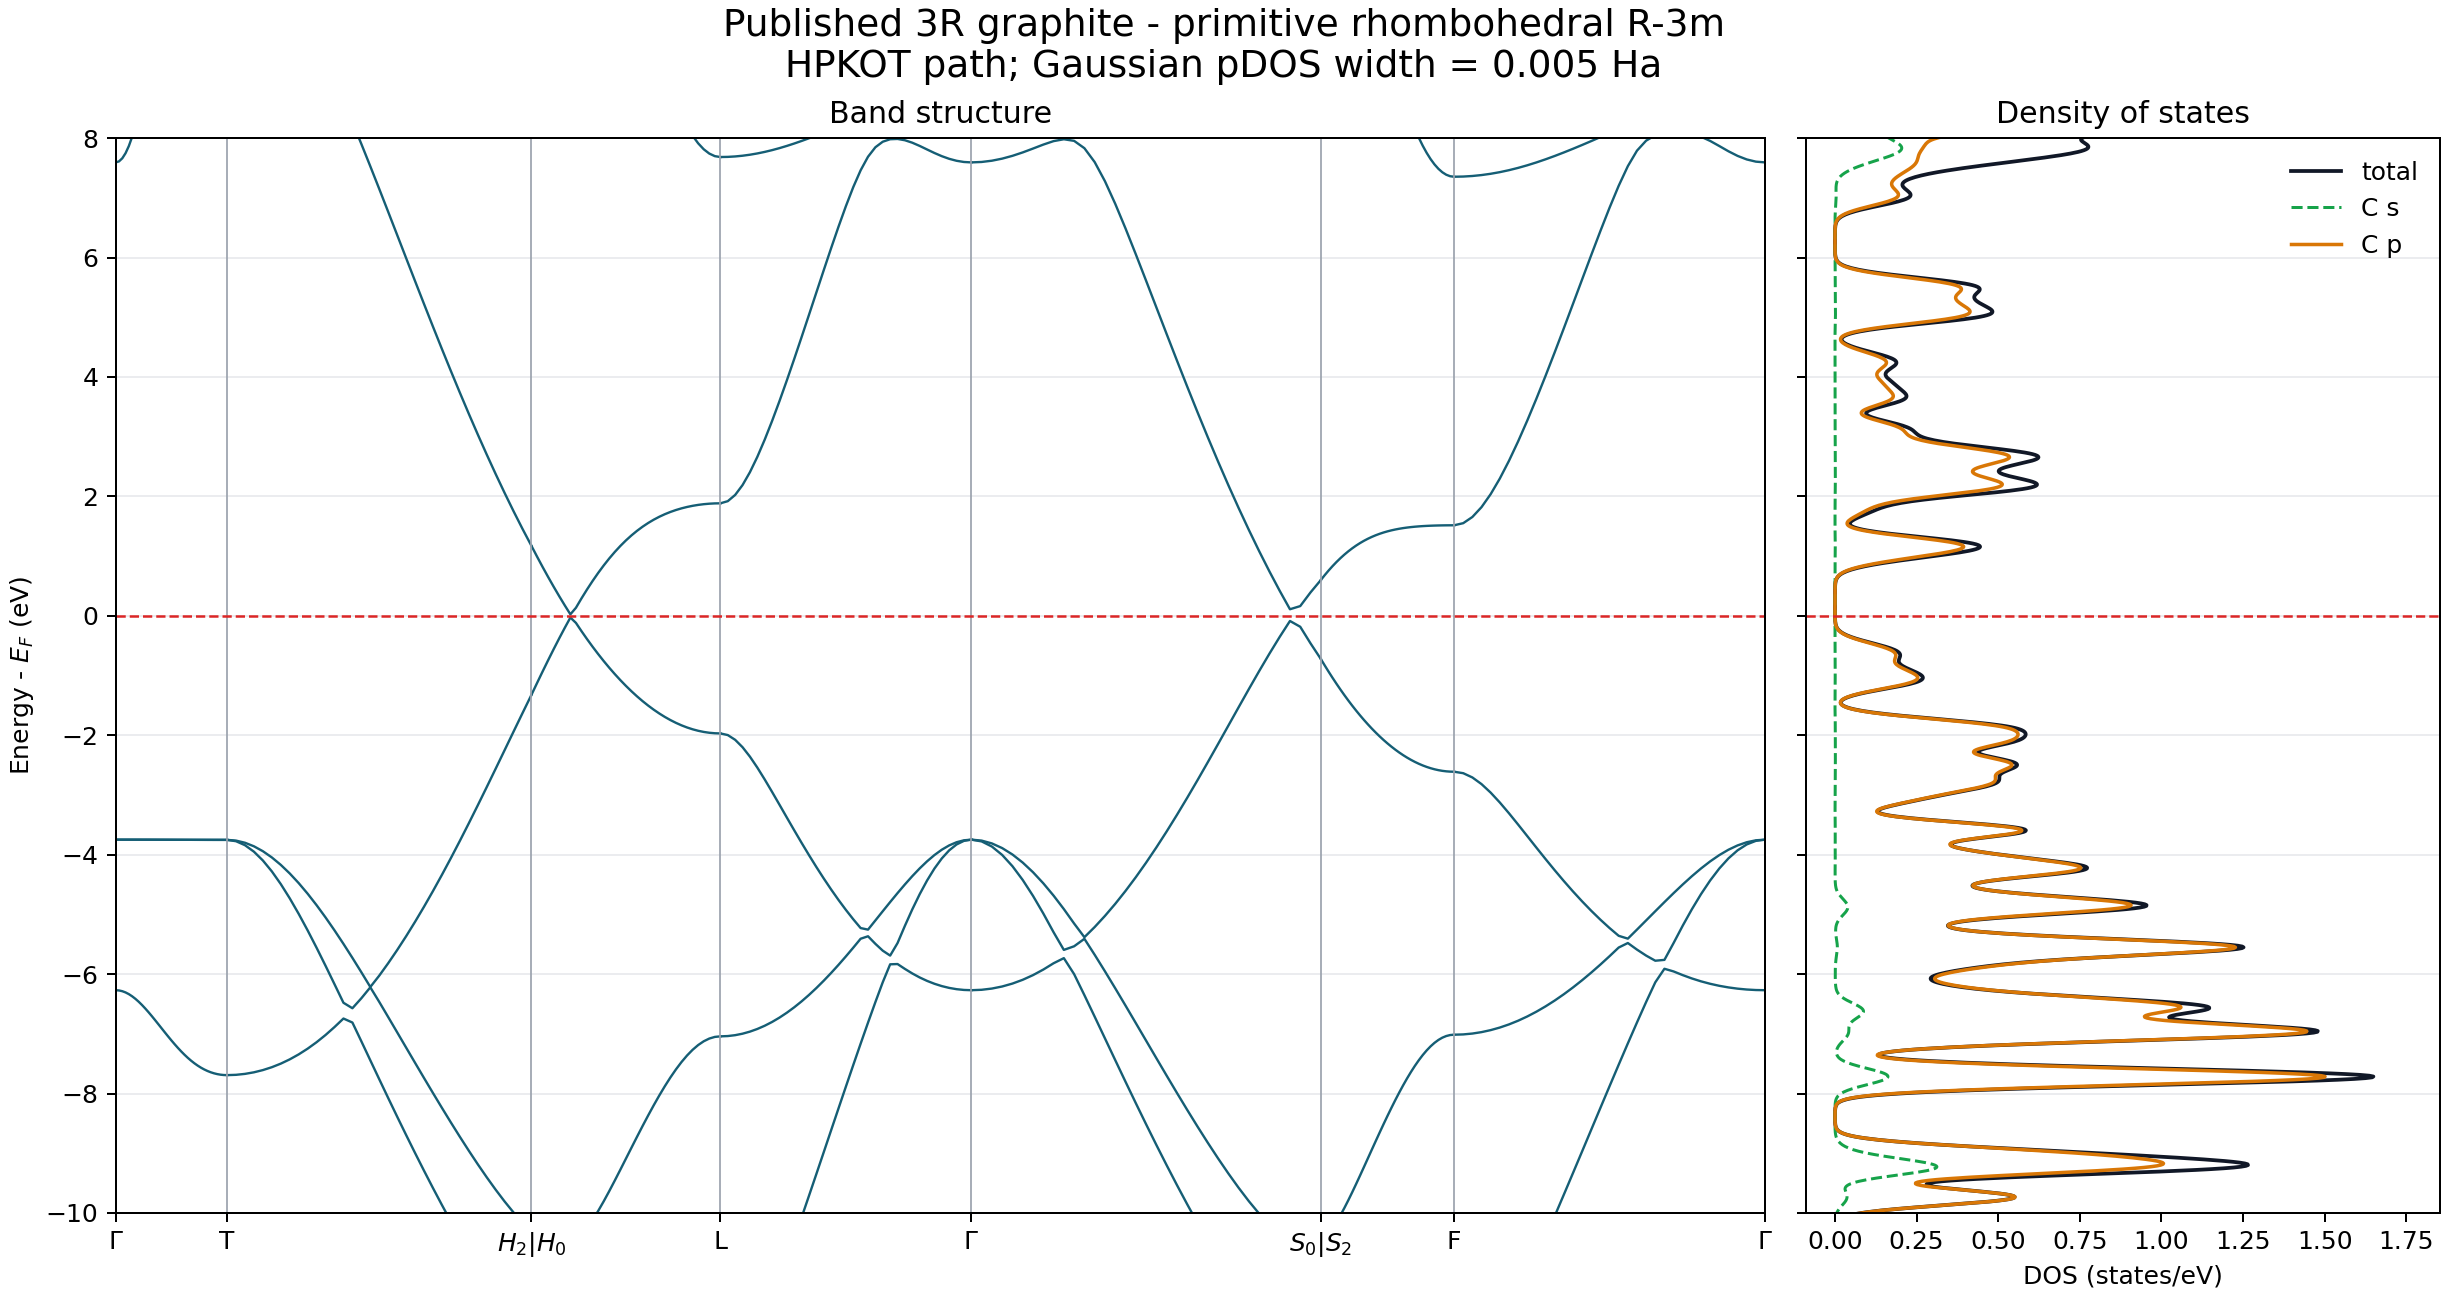
\includegraphics[width=.66\textwidth]{figures/rhombohedral_graphite_band_pdos.png}
\caption{Test 024. Published 3R graphite in its acute rhombohedral primitive cell. The path contains 241 k points, the integrated electron count is 8.0, and the compact-basis path separation is 0.0538 eV.}
\end{figure*}

\section{Selected quantitative outcomes}
For graphite, coupled Method-2 relaxation reduced the maximum force from 0.03191205 to 0.00019971 Ha/bohr and maximum stress from 22.3003 to 0.0431 GPa in six outer cycles. Primitive Si relaxation reduced the maximum force from 0.00918819 to $9.894\times10^{-5}$ Ha/bohr, and its EOS and direct cell relaxation agreed on the lattice minimum. Rutile oxygen relaxed from $u=0.3120$ to 0.3052583. In 2H-MoS$_2$, sulfur moved from $z=0.6150$ to 0.6211887 and the maximum force fell to 0.00019569 Ha/bohr. Monoclinic ZrO$_2$ ended at 0.00039986 Ha/bohr maximum force.

Equivalent-cell tests cover determinant-one shears, primitive/conventional representations, and rotated PDB restart. Test 027 uses the deliberately stringent 400-Ha cutoff and commensurate $11^3$ conventional/$19^3$ primitive meshes to separate representation correctness from ordinary discretization error. Tests 029, 030, and 032 then isolate sampling bounds, block distance, and face-normal geometry at source level.

\section{Interpretation and limits}
A pass demonstrates agreement with the maintained regression's numerical or structural invariants, not universal convergence for production research. Some low cutoffs and Gamma-only meshes are intentional smoke-test settings. Electronic plots are acceptance artifacts made with compact localized bases. Long-time NPT ensemble statistics, every exchange-correlation/basis combination, spin--orbit coupling, and performance optimization for severely unreduced lattices remain separate validation topics. The exact minimum image prioritizes correctness over optimal asymptotic speed.

\section{Conclusion}
The audit identified useful questions but was not treated as authoritative. Source inspection separated mistaken concerns from concrete defects. The latter were fixed in focused commits and verified by targeted reruns before consolidation. With the official Test-005 macOS initialization fix integrated, all 32 maintained tests pass under the requested three-core ceiling. The most consequential new correction is the partition-consistent fractional wrapping rule, which removes an intermittent triclinic NPT failure at its geometric source.

\appendix
\section{Test-by-test record}
\subsection{Test 001: bulk Si 1proc Diag}
Legacy diagonalization regression for bulk diamond Si. The consolidated run records 8 atoms, MPI ranks 2, and 2.598 s wall time. The representative grid cutoff was 50 Ha and the reciprocal sampling was $2\times2\times2$. Acceptance evidence: \emph{4 passed, 32 deselected in 0.08s; PulayMixSC: Reached SCF tolerance of 0.91858E-06 after 5 iterations}. Status: \textbf{PASS}.

\subsection{Test 002: bulk Si 1proc OrderN}
Legacy linear-scaling regression for the same bulk-Si cell. The consolidated run records 8 atoms, MPI ranks 2, and 9.932 s wall time. The representative grid cutoff was 50 Ha and the reciprocal sampling was $\Gamma$ / O(N). Acceptance evidence: \emph{4 passed, 32 deselected in 0.04s}. Status: \textbf{PASS}.

\subsection{Test 003: bulk BTO polarisation}
Berry-phase/Resta polarization regression for displaced BaTiO3. The consolidated run records 5 atoms, MPI ranks 1, and 18.086 s wall time. The representative grid cutoff was 100 Ha and the reciprocal sampling was $1\times1\times1$. Acceptance evidence: \emph{4 passed, 32 deselected in 0.06s; PulayMixSC: Reached SCF tolerance of 0.76963E-07 after 29 iterations}. Status: \textbf{PASS}.

\subsection{Test 004: isol C2H4 4proc PBE0CRI}
Isolated ethylene PBE0 exact exchange using CRI integrals. The consolidated run records 6 atoms, MPI ranks 2, and 12.238 s wall time. The representative grid cutoff was 90 Ha and the reciprocal sampling was $\Gamma$. Acceptance evidence: \emph{4 passed, 32 deselected in 0.06s; PulayMixSC: Reached SCF tolerance of 0.79157E-07 after 15 iterations}. Status: \textbf{PASS}.

\subsection{Test 005: isol C2H4 4proc PBE0GTO}
Isolated ethylene PBE0 exact exchange using GTO integrals; includes the macOS initialization fix. The consolidated run records 6 atoms, MPI ranks 2, and 56.431 s wall time. The representative grid cutoff was 90 Ha and the reciprocal sampling was $\Gamma$. Acceptance evidence: \emph{4 passed, 32 deselected in 0.06s; PulayMixSC: Reached SCF tolerance of 0.78125E-07 after 14 iterations}. Status: \textbf{PASS}.

\subsection{Test 006: isol C2H4 4proc PBE0ERI}
Isolated ethylene PBE0 exact exchange using ERI integrals. The consolidated run records 6 atoms, MPI ranks 2, and 16.437 s wall time. The representative grid cutoff was 90 Ha and the reciprocal sampling was $\Gamma$. Acceptance evidence: \emph{4 passed, 32 deselected in 0.04s; PulayMixSC: Reached SCF tolerance of 0.79157E-07 after 15 iterations}. Status: \textbf{PASS}.

\subsection{Test 007: isol CH spinpol 1proc PBE0CRI}
Spin-polarized isolated CH PBE0 regression. The consolidated run records 2 atoms, MPI ranks 1, and 228.720 s wall time. The representative grid cutoff was 90 Ha and the reciprocal sampling was $\Gamma$. Acceptance evidence: \emph{4 passed, 32 deselected in 0.06s; PulayMixSC: Reached SCF tolerance of 0.57025E-03 after 4 iterations}. Status: \textbf{PASS}.

\subsection{Test 008: surface dipole}
Surface dipole correction regression. The consolidated run records 3 atoms, MPI ranks 1, and 4.493 s wall time. The representative grid cutoff was 100 Ha and the reciprocal sampling was $1\times1\times1$. Acceptance evidence: \emph{4 passed, 32 deselected in 0.04s; PulayMixSC: Reached SCF tolerance of 0.70722E-08 after 38 iterations}. Status: \textbf{PASS}.

\subsection{Test 009: DFT plus U}
DFT+U diagonalization regression. The consolidated run records 2 atoms, MPI ranks 1, and 188.394 s wall time. The representative grid cutoff was 100 Ha and the reciprocal sampling was $3\times3\times3$. Acceptance evidence: \emph{4 passed, 32 deselected in 0.04s; SCF tolerance: 0.00000100}. Status: \textbf{PASS}.

\subsection{Test 010: graphite monoclinic}
Hexagonal graphite and graphene: SCF, bands, PDOS, and cell relaxation. The consolidated run records 4 atoms, MPI ranks 1, 2, and 194.054 s wall time. The representative grid cutoff was 100--150 (120 electronic) Ha and the reciprocal sampling was $4\times4\times2$; line paths. Acceptance evidence: \emph{Workflow completed successfully!; Error in process 1}. Status: \textbf{PASS}.

\subsection{Test 011: hfo2}
Monoclinic HfO2: Ewald force/stress, equivalent cells, relaxation, bands, and PDOS. The consolidated run records 12 atoms, MPI ranks 1, 2, and 63.228 s wall time. The representative grid cutoff was 80--200 (100 electronic) Ha and the reciprocal sampling was $1^3$, $2^3$, $3^3$; line path. Acceptance evidence: \emph{[1/4] Converged PBE/DZP SCF density on monoclinic HfO2; SCF tolerance: 0.00001000}. Status: \textbf{PASS}.

\subsection{Test 012: bulk Si primitive nonorthogonal}
Two-atom primitive diamond Si: relaxation, EOS, six strains, bands, and PDOS. The consolidated run records 2 atoms, MPI ranks 1, and 47.383 s wall time. The representative grid cutoff was 80 Ha and the reciprocal sampling was $4^3$, $6^3$, $8^3$, $10^3$; line path. Acceptance evidence: \emph{[2/5] Converged self-consistent density}. Status: \textbf{PASS}.

\subsection{Test 013: rutile TiO2 tetragonal}
Rutile TiO2 orthogonal-anisotropic control with relaxation, bands, and PDOS. The consolidated run records 6 atoms, MPI ranks 1, 2, and 153.657 s wall time. The representative grid cutoff was 100 Ha and the reciprocal sampling was $3\times3\times5$ to $5\times5\times7$; line path. Acceptance evidence: \emph{[2/5] Converged SCF density}. Status: \textbf{PASS}.

\subsection{Test 014: bulk 2h mos2 hexagonal}
Bulk 2H-MoS2: hexagonal relaxation, bands, and orbital-resolved PDOS. The consolidated run records 6 atoms, MPI ranks 1, 2, and 177.726 s wall time. The representative grid cutoff was 100 Ha and the reciprocal sampling was $4\times4\times2$ to $6\times6\times3$; line path. Acceptance evidence: \emph{PASS: sulfur internal relaxation converged; MaxF 0.02736401 -> 0.00019562 Ha/a0.; [2/5] Converged relaxed-cell SCF density}. Status: \textbf{PASS}.

\subsection{Test 015: monoclinic zro2}
Monoclinic ZrO2: symmetry restoration, relaxation, bands, and PDOS. The consolidated run records 12 atoms, MPI ranks 1, 3, and 719.721 s wall time. The representative grid cutoff was 100 Ha and the reciprocal sampling was $3^3$ to $5^3$; line path. Acceptance evidence: \emph{[2/5] Symmetry restoration and converged SCF density}. Status: \textbf{PASS}.

\subsection{Test 016: exact minimum image triclinic}
Exact Euclidean minimum image in adversarial triclinic and unreduced cells. The consolidated run records no atom input (source-level geometry test), MPI ranks --, and 0.734 s wall time. The representative grid cutoff was -- Ha and the reciprocal sampling was source-level. Acceptance evidence: \emph{the maintained numerical and structural acceptance gates completed}. Status: \textbf{PASS}.

\subsection{Test 017: nonorthogonal polarisation extxyz}
Equivalent-cell polarization and full extended-XYZ lattice/stress metadata. The consolidated run records 2 atoms, MPI ranks 1, and 10.916 s wall time. The representative grid cutoff was 120 Ha and the reciprocal sampling was $1\times1\times1$. Acceptance evidence: \emph{the maintained numerical and structural acceptance gates completed}. Status: \textbf{PASS}.

\subsection{Test 018: nonorthogonal vdw graphene}
Nonlocal vdW-DFT invariance under a determinant-one graphene basis change. The consolidated run records 2 atoms, MPI ranks 1, and 7.142 s wall time. The representative grid cutoff was 80 Ha and the reciprocal sampling was $1\times1\times1$. Acceptance evidence: \emph{the maintained numerical and structural acceptance gates completed}. Status: \textbf{PASS}.

\subsection{Test 019: nonorthogonal npt md}
Nonorthogonal variable-cell MD and partition-consistent triclinic wrapping. The consolidated run records 2 atoms, MPI ranks 1, and 22.171 s wall time. The representative grid cutoff was 80 Ha and the reciprocal sampling was $1\times1\times1$. Acceptance evidence: \emph{the maintained numerical and structural acceptance gates completed}. Status: \textbf{PASS}.

\subsection{Test 020: extreme skew sfc mpi}
Extreme-skew space-filling-curve decomposition and MPI invariance. The consolidated run records 2 atoms, MPI ranks 1, and 40.301 s wall time. The representative grid cutoff was 80 Ha and the reciprocal sampling was $2\times2\times2$. Acceptance evidence: \emph{the maintained numerical and structural acceptance gates completed}. Status: \textbf{PASS}.

\subsection{Test 021: hfo2 full cell npt}
Six-degree-of-freedom full-cell NPT dynamics for monoclinic HfO2. The consolidated run records 12 atoms, MPI ranks 3, and 49.975 s wall time. The representative grid cutoff was 80 Ha and the reciprocal sampling was $1\times1\times1$. Acceptance evidence: \emph{the maintained numerical and structural acceptance gates completed}. Status: \textbf{PASS}.

\subsection{Test 022: graphene xy npt}
In-plane symmetric NPT dynamics for a 3x3 graphene slab. The consolidated run records 18 atoms, MPI ranks 3, and 41.089 s wall time. The representative grid cutoff was 80 Ha and the reciprocal sampling was $1\times1\times1$. Acceptance evidence: \emph{the maintained numerical and structural acceptance gates completed}. Status: \textbf{PASS}.

\subsection{Test 023: hcp zr method3 relax}
Coupled fixed-angle Method-3 relaxation of HCP Zr. The consolidated run records 2 atoms, MPI ranks 1, and 192.464 s wall time. The representative grid cutoff was 100 Ha and the reciprocal sampling was $6\times6\times4$. Acceptance evidence: \emph{the maintained numerical and structural acceptance gates completed}. Status: \textbf{PASS}.

\subsection{Test 024: rhombohedral graphite sfc mpi}
Published 3R graphite: SFC, MPI, Ewald, bands, and PDOS. The consolidated run records 2 atoms, MPI ranks 1, 2, and 30.180 s wall time. The representative grid cutoff was 60 Ha and the reciprocal sampling was $2^3$ static; $8^3$ electronic; line path. Acceptance evidence: \emph{the maintained numerical and structural acceptance gates completed}. Status: \textbf{PASS}.

\subsection{Test 025: blip basis smoke}
Orthorhombic Si blip-basis smoke test. The consolidated run records 8 atoms, MPI ranks 2, and 2.545 s wall time. The representative grid cutoff was 50 Ha and the reciprocal sampling was $2\times2\times2$. Acceptance evidence: \emph{the maintained numerical and structural acceptance gates completed}. Status: \textbf{PASS}.

\subsection{Test 026: nonorthogonal blip basis}
Equivalent nonorthogonal Si blip-basis regression. The consolidated run records 8 atoms, MPI ranks 1, 2, and 37.614 s wall time. The representative grid cutoff was 50 Ha and the reciprocal sampling was $2\times2\times2$. Acceptance evidence: \emph{the maintained numerical and structural acceptance gates completed}. Status: \textbf{PASS}.

\subsection{Test 027: si equivalent cells}
High-accuracy primitive/conventional diamond-Si energy and stress equivalence. The consolidated run records 2 atoms, MPI ranks 1, and 123.092 s wall time. The representative grid cutoff was 400 Ha and the reciprocal sampling was $11^3$ cubic; $19^3$ primitive. Acceptance evidence: \emph{the maintained numerical and structural acceptance gates completed}. Status: \textbf{PASS}.

\subsection{Test 028: auto full stress}
Automatic activation and parsing of the full stress tensor for general cells. The consolidated run records 2 atoms, MPI ranks 1, and 3.786 s wall time. The representative grid cutoff was 80 Ha and the reciprocal sampling was $2\times2\times2$. Acceptance evidence: \emph{the maintained numerical and structural acceptance gates completed}. Status: \textbf{PASS}.

\subsection{Test 029: general cell sampling}
FFT and automatically generated k-point sampling bounds for an extreme cell. The consolidated run records 2 atoms, MPI ranks 1, and 3.378 s wall time. The representative grid cutoff was 20 Ha and the reciprocal sampling was automatic density rule. Acceptance evidence: \emph{PASS: FFT cutoff sphere is contained and automatic k-point spacing uses reciprocal-vector norms}. Status: \textbf{PASS}.

\subsection{Test 030: triclinic block distance}
Exact point-to-parallelepiped distance for triclinic integration-grid blocks. The consolidated run records no atom input (source-level geometry test), MPI ranks --, and 0.525 s wall time. The representative grid cutoff was -- Ha and the reciprocal sampling was source-level. Acceptance evidence: \emph{the maintained numerical and structural acceptance gates completed}. Status: \textbf{PASS}.

\subsection{Test 031: rotated triclinic pdb}
Rotated triclinic PDB write/restart preserving orientation through SCALE records. The consolidated run records 2 atoms, MPI ranks 1, and 4.034 s wall time. The representative grid cutoff was 80 Ha and the reciprocal sampling was $2\times2\times2$. Acceptance evidence: \emph{maximum lattice error (Angstrom): 8.918e-06; maximum fractional-coordinate error: 1.540e-04}. Status: \textbf{PASS}.

\subsection{Test 032: triclinic surface geometry}
Face area, normal height, and dipole-coordinate geometry for triclinic slabs. The consolidated run records no atom input (source-level geometry test), MPI ranks --, and 0.418 s wall time. The representative grid cutoff was -- Ha and the reciprocal sampling was source-level. Acceptance evidence: \emph{the maintained numerical and structural acceptance gates completed}. Status: \textbf{PASS}.

\section{Reproducibility record}
Report source commit before adding this artifact: \code{f527e5660224}. Consolidated run: \code{testsuite/test\_runs/20260809-235347/summary.json}, assembled from the full sweep \code{20260809-230103} plus successful targeted reruns of Tests 011, 019, and 027. The shipped \code{data/all\_tests\_summary.json} is an immutable copy used to generate the tables. The report generator copies only maintained figures and writes the REV\TeX\ source and bibliography in this folder.

\bibliography{references}
\end{document}
